\documentclass{beamer}
\mode<presentation> {

% The Beamer class comes with a number of default slide themes
% which change the colors and layouts of slides. Below this is a list
% of all the themes, uncomment each in turn to see what they look like.

%\usetheme{default}
%\usetheme{AnnArbor}
%\usetheme{Antibes}
%\usetheme{Bergen}
%\usetheme{Berkeley}
%\usetheme{Berlin}
%\usetheme{Boadilla}
%\usetheme{CambridgeUS}
%\usetheme{Copenhagen}
%\usetheme{Darmstadt}
%\usetheme{Dresden}
%\usetheme{Frankfurt}
%\usetheme{Goettingen}
%\usetheme{Hannover}
%\usetheme{Ilmenau}
%\usetheme{JuanLesPins}
%\usetheme{Luebeck}
\usetheme{Madrid}
%\usetheme{Malmoe}
%\usetheme{Marburg}
%\usetheme{Montpellier}
%\usetheme{PaloAlto}
%usetheme{Pittsburgh}
%\usetheme{Rochester}
%\usetheme{Singapore}
%\usetheme{Szeged}
%\usetheme{Warsaw}

% As well as themes, the Beamer class has a number of color themes
% for any slide theme. Uncomment each of these in turn to see how it
% changes the colors of your current slide theme.

%\usecolortheme{albatross}
%\usecolortheme{beaver}
%\usecolortheme{beetle}
%\usecolortheme{crane}
%\usecolortheme{dolphin}
%\usecolortheme{dove}
%\usecolortheme{fly}
%\usecolortheme{lily}
%\usecolortheme{orchid}
%\usecolortheme{rose}
%\usecolortheme{seagull}
%\usecolortheme{seahorse}
%\usecolortheme{whale}
%\usecolortheme{wolverine}

%\setbeamertemplate{footline} % To remove the footer line in all slides uncomment this line
%\setbeamertemplate{footline}[page number] % To replace the footer line in all slides with a simple slide count uncomment this line

%\setbeamertemplate{navigation symbols}{} % To remove the navigation symbols from the bottom of all slides uncomment this line
}

\usepackage{graphicx} % Allows including images
\usepackage{booktabs} % Allows the use of \toprule, \midrule and \bottomrule in tables
\usepackage{fancyvrb}

\usepackage{array}
% Support allignment and newlines in table cells
\newcolumntype{L}[1]{>{\raggedright\let\newline\\\arraybackslash\hspace{0pt}}m{#1}}
\newcolumntype{C}[1]{>{\centering\let\newline\\\arraybackslash\hspace{0pt}}m{#1}}
\newcolumntype{R}[1]{>{\raggedleft\let\newline\\\arraybackslash\hspace{0pt}}m{#1}}


\newenvironment{hanging}
   { \par
     \vspace{0.2cm}
     \parskip 0.2cm
     \leftskip 1.5cm
     \parindent -0.75cm
     \par
   }
   { \par
     \leftskip 0.0cm
     \parindent 0.0cm
     \parskip 0.0cm
     \vspace{0.2cm}
   }

%----------------------------------------------------------------------------------------
%  TITLE PAGE
%----------------------------------------------------------------------------------------

\title[TrickHLA]{TrickHLA v3}
\subtitle{An HLA interface package for Trick}

\author[Crues,Dexter]{Edwin Z. Crues, Ph.D. \\ Daniel E. Dexter}
\institute[NASA JSC] % Your institution as it will appear on the bottom of every slide, may be shorthand to save space
{
Simulation and Graphics Branch (ER7)\\
NASA Johnson Space Center \\
2101 NASA Parkway, Houston, Texas, 77058\\
\medskip
\texttt{edwin.z.crues@nasa.gov}\\
\texttt{daniel.e.dexter@nasa.gov}
}
%\date{\today}
\date{January 2021}

%------------------------------------------------

\graphicspath{ {./figures/} }

\begin{document}

   \begin{frame}
      \titlepage
   \end{frame}

   \begin{frame}
      \frametitle{Outline}
      \tableofcontents
   \end{frame}
   
   \section{Introduction}
   
   \begin{frame}
      \frametitle{Introduction}
      \begin{itemize}
         \item The main design goal of TrickHLA is to allow existing Trick simulations to use the IEEE-1516 High Level Architecture (HLA) with minimal development effort.
         \item TrickHLA is an HLA abstraction for the Trick simulation environment.
         \item TrickHLA is data driven and provides a simple API for the HLA functionality.
         \item TrickHLA is available from the Trick website http://trick.jsc.nasa.gov/
      \end{itemize}
   \end{frame}
   
   \section{Minimum Software Requirements}
   
   \begin{frame}
      \frametitle{Minimum Software Requirements}
      \begin{itemize}
         \item Trick version 17 or newer.
         \item IEEE-1516-2010 HLA standard compliant Runtime Infrastructure (RTI).
         \item TrickHLA callback interfaces must be written in C++.
      \end{itemize}
   \end{frame}
   
   \section{TrickHLA Features}

   \begin{frame}
      \frametitle{TrickHLA Features}
      \begin{center}
      \Huge{TrickHLA Features}
      \end{center}
   \end{frame}
   
   \begin{frame}
      \frametitle{TrickHLA Features}
      \begin{itemize}
         \item Primitive C/C++ data types.
         \item Static arrays of primitive data types.
         \item One-dimensional dynamic arrays of primitive data types.
         \item Strings and static arrays of strings.
         \item Opaque (hidden type) data.
         \item Automatically encodes/decodes the data to/from the RTI using the specified HLA encoding.
         \item Big/Little Endian for primitives
         \item HLAunicodeString, HLAASCIIstring, and HLAopaqueData for strings (i.e. char *)
         \item User defined packing and unpacking functions to allow for data transformations before data is sent to (pack) or after data is received from (unpack) the other federates.
         \item Automatically handles HLA time advancement.
      \end{itemize}
   \end{frame}
   
   \begin{frame}
      \frametitle{TrickHLA Features}
      \framesubtitle{Continued}
      \begin{itemize}
         \item Handles real time and non-real time simulations
         \item Lag Compensation
         \begin{itemize}
            \item None
            \item Sending-side
            \item Receive-side
            \end{itemize}
         \item Interactions (job safe and thread safe)
         \begin{itemize}
            \item Receive Order (RO)
            \item Timestamp Order (TSO)
         \end{itemize}
         \item Ownership Transfer
         \item Multiphase Initialization, which allows simulation initialization data to be shared between federates before the simulation starts. This includes a simulation configuration object.
         \item Automatically synchronizes the startup of a distributed simulation without depending on specific federate start order.
      \end{itemize}
   \end{frame}
   
   \begin{frame}
      \frametitle{TrickHLA Features}
      \framesubtitle{Continued}
      \begin{itemize}
         \item Coordinated Federation Save \& Restore.
         \item Late joining federates.
         \item Supports IEEE-1516.1-2000, and IEEE-1516.1-2010 (a.k.a HLA Evolved).
         \item Allows subscription to non-required federate data.
         \item Attribute preferred order (Receive or Timestamp Order) can be overridden.
         \item Blocking cyclic data reads (only 2 federate case supported for now).
         \item Notification of object deletions.
      \end{itemize}
   \end{frame}
   
   \section{Setting up the Environment}

   \begin{frame}
      \frametitle{Setting up the Environment}
      \begin{center}
      \Huge{Setting up the Environment}
      \end{center}
   \end{frame}
   
   \begin{frame}[fragile]
      \frametitle{Setting up the Environment}
      \begin{itemize}
         \item Set the path to the TrickHLA directory
         \begin{itemize}
            \item Set the environment variable \texttt{TRICKHLA\_HOME} to the system file path for the TrickHLA source directory.
            \item For example:
\begin{Verbatim}[frame=single]
setenv TRICKHLA_HOME ${HOME}/Trick/hla/TrickHLA
\end{Verbatim}
         \end{itemize}
         \item Add the TrickHLA models directory to the Trick compile environment
         \begin{itemize}
            \item The Trick environment variable \texttt{TRICK\_CXXFLAGS} must include the path to the TrickHLA models.
            \item For example:
\begin{Verbatim}[frame=single]
TRICK_CXXFLAGS += -I${TRICKHLA_HOME}/models
\end{Verbatim}
         \end{itemize}
      \end{itemize}
   \end{frame}
   
   \begin{frame}[fragile]
      \frametitle{Setting up the Environment}
      \framesubtitle{Setting up a C-Shell environment}
      \begin{itemize}
         \item Set up the RTI for a C-Shell environment
         \begin{itemize}
            \item Copy the provided scripts \texttt{/.rti\_cshrc} file to your home directory.
            \item Change the \texttt{RTI\_HOME} environment variable in the \texttt{.rti\_cshrc} file to point to the location of your RTI installation.
            \item For example:
\begin{Verbatim}[frame=single]
setenv RTI_HOME ${HOME}/rti/prti1516e_v5.5.1
\end{Verbatim}
            \item Add the following lines to your \texttt{.Trick\_user\_cshrc} file in your home directory.
\begin{Verbatim}[frame=single]
# Perform RTI setup, which MUST occur after you set
# up your TRICK_CXXFLAGS since .rti_cshrc will appended
# entries to it.
if ( -e ${HOME}/.rti_cshrc ) then
   source ${HOME}/.rti_cshrc
endif
\end{Verbatim}
         \end{itemize}
      \end{itemize}
   \end{frame}
   
   \begin{frame}[fragile]
      \frametitle{Setting up the Environment}
      \framesubtitle{Setting up a Bourne Shell environment}
      \begin{itemize}
         \item Set up the RTI Bourne Shell environment
         \begin{itemize}
            \item Copy the provided scripts \texttt{/.rti\_profile} file to your home directory.
            \item Change the \texttt{RTI\_HOME} environment variable in the \texttt{.rti\_profile} file to point to the location of your RTI installation.
            \item For example:
\begin{Verbatim}[frame=single]
set RTI_HOME=${HOME}/rti/prti1516e_v5.5.1
export RTI_HOME
\end{Verbatim}
            \item Add the following lines to your \texttt{.Trick\_profile} file in your home directory.
\begin{Verbatim}[frame=single]
# Perform RTI setup, which MUST occur after you set
# up your TRICK_CXXFLAGS since .rti_profile will appended
# entries to it.
if [ -f ${HOME}/.rti_profile ] ; then
. ${HOME}/.rti_profile
fi
\end{Verbatim}
         \end{itemize}
      \end{itemize}
   \end{frame}
   
   \section{Sine Wave Simulation Example}

   \begin{frame}
      \frametitle{Sine Wave Simulation Example}
      \begin{center}
      \Huge{Sine Wave Simulation Example}
      \end{center}
   \end{frame}
   
   \begin{frame}
      \frametitle{Sine Wave Simulation Example}
      \begin{itemize}
         \item A simple simulation of a sinusoid will be used to describe the TrickHLA concepts.
         \item The example can be found in \texttt{\$\{TRICKHLA\_HOME\}/sims/TrickHLA/SIM\_sine}.
         \item Equation of a sinusoid with a given amplitude $a$, angular frequency $\omega$ (period $2\pi/\omega$), and phase $\phi$: $f(t) = a \sin( \omega t + \phi )$
      \end{itemize}

      \begin{small}
      \begin{center}
      \begin{tabular}{ |l|c|c| } \hline
       \bf{Sinusoidal Parameter} & \bf{Analytic} & \bf{Propagated} \\ \hline
       Amplitude & 2 & 1 \\ \hline
       Frequency & 0.1963 & 0.3927 \\ \hline
       Period & 32 & 16 \\ \hline
      \end{tabular}
      \end{center}
      \end{small}

      \begin{center}
      \begin{figure}
      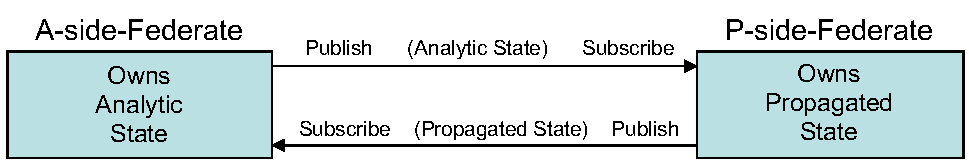
\includegraphics[scale=0.65]{TutorialFig1.pdf}
      \end{figure}
      \end{center}
      
   \end{frame}
   
   \section{Steps to Adding TrickHLA to a Trick Simulation}

   \begin{frame}
      \frametitle{Steps to Adding TrickHLA to a Trick Simulation}
      \begin{center}
      \Huge{Steps to Adding TrickHLA to a Trick Simulation}
      \end{center}
   \end{frame}
   
   \begin{frame}
      \frametitle{Steps to Adding TrickHLA to a Trick Simulation}
      \begin{itemize}
      \item Adding TrickHLA to a Trick simulation consists of three steps.
      \end{itemize}
      \begin{hanging}
      Step 1: Add the provided TrickHLA specific \texttt{THLA.sm} simulation
      module to your \texttt{S\_define} file, and pass in the \texttt{data\_cycle}
      and \texttt{interaction\_cycle} parameter values, using the \texttt{
      THLA\_DATA\_CYCLE\_TIME} and \texttt{THLA\_INTERACTION\_CYCLE\_TIME}
      values defined at the top of the \texttt{S\_define} file.
      
      Step 2: Add a generic \texttt{THLA\_INIT} multiphase initialization sim
      object to your \texttt{S\_define} file, and pass in the \texttt{TrickHLA::Manager}
      and \texttt{TrickHLA::Federate} objects from \texttt{THLA.sm}.
      
      Step 3: Configure TrickHLA through settings in your simulation RUN \texttt{input.py} file.
      \end{hanging}
      
   \end{frame}
   
   \begin{frame}[fragile]
      \frametitle{Steps to Adding TrickHLA to a Trick Simulation}
      \framesubtitle{Step 1: THLA Simulation Object}
      \begin{itemize}
         \item Add to your S\_define file:
\begin{Verbatim}[frame=single, fontsize=\tiny]
// Define HLA job cycle times:
#define THLA_DATA_CYCLE_TIME         0.250  // HLA data communication cycle time.
#define THLA_INTERACTION_CYCLE_TIME  0.050  // HLA Interaction cycle time.

// get sim object for generalized TrickHLA interface routines:
#include ”../../../../shared/trick10/S_modules/THLA.sm”
THLASimObject THLA( THLA_DATA_CYCLE_TIME, THLA_INTERACTION_CYCLE_TIME);
\end{Verbatim}
         \item \texttt{THLA\_DATA\_CYCLE\_TIME} defines the rate at which data is
         exchanged through the RTI.
         \item \texttt{THLA\_INTERACTION\_CYCLE\_TIME} defines the rate at which
         received Interactions in Receive-Order (RO) will be serviced.
         \item Each of the above two values must be an integer multiple of Trick’s
         real-time frame (i.e., the $n$ value set via
         \texttt{trick.exec\_set\_software\_frame($n$)} ). 
      \end{itemize}
   \end{frame}
   
   \begin{frame}
      \frametitle{Steps to Adding TrickHLA to a Trick Simulation}
      \framesubtitle{TrickHLA jobs in THLA.sm}
      \begin{figure}
      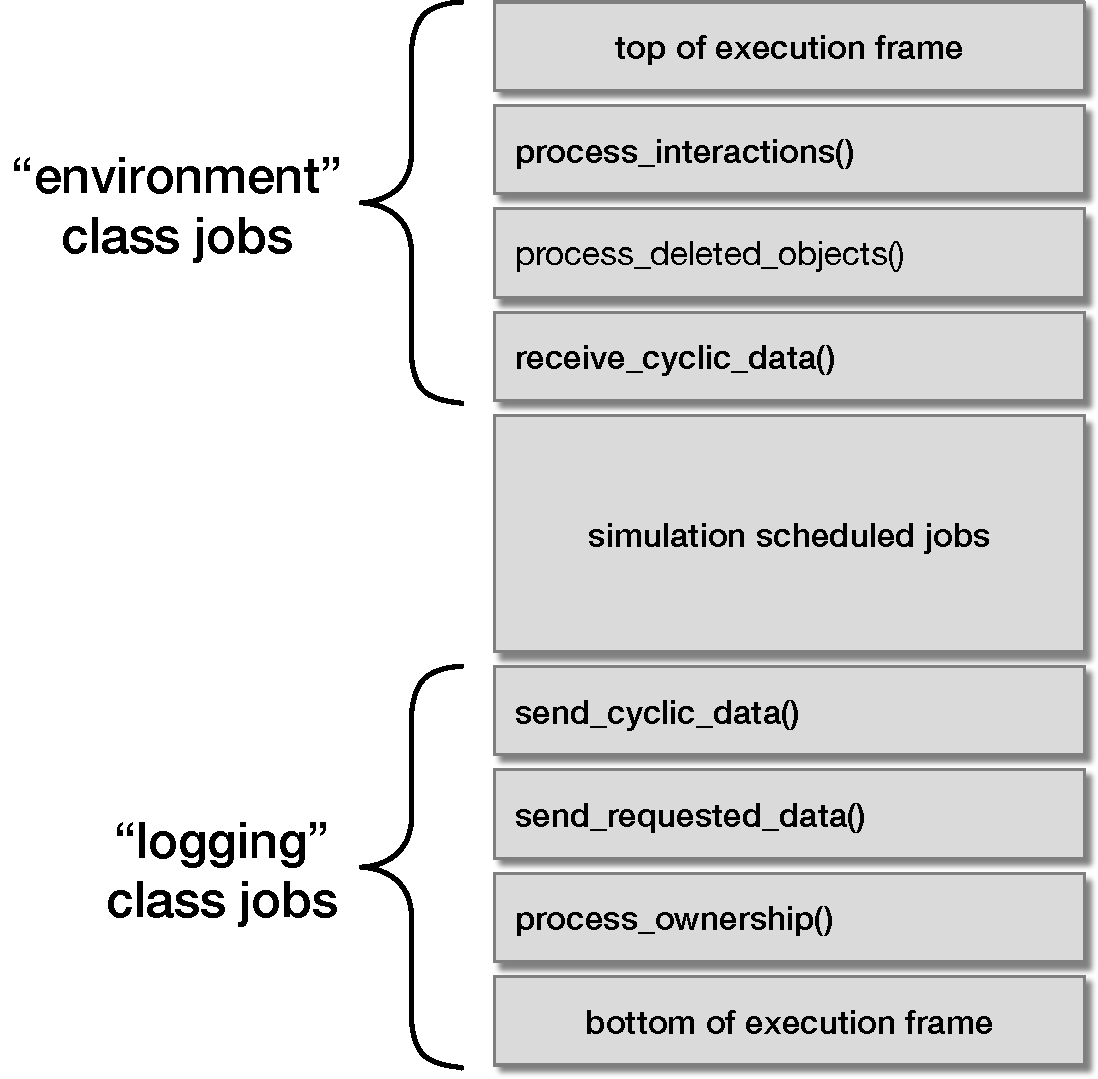
\includegraphics[scale=0.4]{TutorialTHLAJobs.pdf}
      \end{figure}
   \end{frame}
   
   \begin{frame}[fragile]
      \frametitle{Steps to Adding TrickHLA to a Trick Simulation}
      \framesubtitle{Step 2: THLA\_INIT Simulation Object}
      \begin{itemize}
         \item Add to your S\_define file:
      \end{itemize}
\begin{Verbatim}[frame=single, fontsize=\tiny]
##include "simconfig/include/SimpleSimConfig.hh”
class THLAInitSimObject : public Trick::SimObject {
  public:
    SimpleSimConfig simple_sim_config; // The simple simulation configuration
    THLAInitSimObject( TrickHLAManager  & thla_mngr,
                       TrickHLAFederate & thla_fed )
       : thla_manager( thla_mngr ), thla_federate( thla_fed )
    {
       // Make sure we initialize the sim config before the TrickHLAManager
       P1 ("initialization") simple_sim_config.initialize(
                                       thla_federate.known_feds_count,
                                       thla_federate.known_feds ); 
       // Send all the initialization data
       P100 ("initialization") thla_manager.send_init_data();
       // Wait to receive all the initialization data
       P100 ("initialization") thla_manager.receive_init_data();
       // Clear remaining initialization sync-points
       P100 ("initialization") thla_manager.clear_init_sync_points();
  private:
    TrickHLAManager  & thla_manager;
    TrickHLAFederate & thla_federate;
    THLAInitSimObject(const THLAInitSimObject & rhs); // do not allow copy
    THLAInitSimObject & operator=(const THLAInitSimObject & rhs); // do not allow assign
    THLAInitSimObject();  // do not allow default constructor
};
THLAInitSimObject THLA_INIT( THLA.manager, THLA.federate );
\end{Verbatim}
   \end{frame}
   
   \begin{frame}
      \frametitle{Steps to Adding TrickHLA to a Trick Simulation}
      \framesubtitle{Step 3: Configuring TrickHLA}
      \begin{itemize}
         \item The last step to adding TrickHLA to a simulation is to configure
         it through settings in your input.py file.
         \item The majority of the presentation will cover TrickHLA configuration for:
      \begin{enumerate}
         \item General Configuration
         \item Multiphase Initialization
         \item Data Packing and Unpacking
         \item Interactions
         \item Ownership Transfer
         \item Lag Compensation
         \item Object Deletion 
      \end{enumerate}
      \end{itemize}
   \end{frame}
   
      \section{General TrickHLA Configuration}

   \begin{frame}
      \frametitle{General TrickHLA Configuration}
      \begin{center}
      \Huge{General TrickHLA Configuration}
      \end{center}
   \end{frame}
   
   \begin{frame}
      \frametitle{General TrickHLA Configuration}
      General TrickHLA configuration consists of the following:
      \begin{enumerate}
         \item General TrickHLA Configuration
         \item Initializing the Federate
         \item Initializing the List of Known Federates
         \item Initializing the Debug Level (Optional)
         \item Initializing the Data Objects
         \item Initializing the Data Object Attributes
      \end{enumerate}
   \end{frame}
   
   \begin{frame}[fragile]
      \frametitle{General TrickHLA Configuration}
      \framesubtitle{Initializing the Central RTI Component Settings}
      \begin{itemize}
         \item The Pitch Central RTI Component (CRC) is initialized by specifying
         the host, port, and lookahead time as shown below. The host and port
         describe where the CRC is/will be running.
         \item Notice the settings are based on the simulation object name and
         the parameter name as they exist in the \texttt{S\_define} file.
         \item In the \texttt{RUN\_a\_side/input.py} file:
      \end{itemize}
\begin{Verbatim}[frame=single, fontsize=\footnotesize]
# Configure the CRC for the Pitch RTI.
THLA.federate.local_settings = "crcHost = localhost\n crcPort = 8989”
THLA.federate.lookahead_time = 0.25  # this is THLA_DATA_CYCLE_TIME
\end{Verbatim}
   \end{frame}
   
   \begin{frame}[fragile]
      \frametitle{General TrickHLA Configuration}
      \framesubtitle{Initializing the Federate}
      \begin{itemize}
         \item The input.py file settings determine how each federate shares data.
\begin{Verbatim}[frame=single, fontsize=\footnotesize]
In the RUN_a_side/input.py file:
THLA.federate.name                  = "A-side-Federate"
THLA.federate.enable_FOM_validation = False
THLA.federate.FOM_modules           = 
   "S_FOMfile.xml,TrickHLAFreezeInteraction.xml"
THLA.federate.federation_name       = "SineWaveSim"
THLA.federate.time_regulating       = True
THLA.federate.time_constrained      = True
\end{Verbatim}
         \item In the \texttt{RUN\_p\_side/input.py} file:
\begin{Verbatim}[frame=single, fontsize=\footnotesize]
THLA.federate.name                  = "P-side-Federate"
THLA.federate.enable_FOM_validation = False
THLA.federate.FOM_modules           = 
   "S_FOMfile.xml,TrickHLAFreezeInteraction.xml"
THLA.federate.federation_name       = "SineWaveSim"
THLA.federate.time_regulating       = True
THLA.federate.time_constrained      = True
\end{Verbatim}
      \end{itemize}
   \end{frame}
   
   \begin{frame}[fragile]
      \frametitle{General TrickHLA Configuration}
      \framesubtitle{Initializing the List of Known Federates}
      \begin{itemize}
         \item A list of federates known to be in the federation is initialized next.
         \item The simulation will wait for all federates designated as “required”
         to join the simulation before continuing on. These required federates
         define the distributed simulation parts that MUST exist for the
         simulation to run.
         \item In both the \texttt{RUN\_a\_side/input.py} and \texttt{RUN\_p\_side\_input.py} files:
\begin{Verbatim}[frame=single, fontsize=\footnotesize]
THLA.federate.enable_known_feds      = True
THLA.federate.known_feds_count       = 2
THLA.federate.known_feds             = trick.alloc_type(
   THLA.federate.known_feds_count, "TrickHLAKnownFederate" )
THLA.federate.known_feds[0].name     = "A-side-Federate"
THLA.federate.known_feds[0].required = True
THLA.federate.known_feds[1].name     = "P-side-Federate"
THLA.federate.known_feds[1].required = True
\end{Verbatim}
      \end{itemize}
   \end{frame}
   
   \begin{frame}[fragile]
      \frametitle{General TrickHLA Configuration}
      \framesubtitle{Initializing the Debug Level (Optional)}
      \begin{itemize}
         \item Although not required, it is recommended that you enable TrickHLA
         debug messages while you are getting your simulation to work with
         TrickHLA for the first time.
         \item Varying amounts of messages may be output by setting the debug
         level, which ranges from \texttt{THLA\_LEVEL0\_TRACE} (no messages) to
         \texttt{THLA\_LEVEL11\_TRACE} (all messages).
         \item For example:
\begin{Verbatim}[frame=single, fontsize=\footnotesize]
THLA.manager.debug_handler.debug_level = trick.THLA_LEVEL3_TRACE
\end{Verbatim}
      \end{itemize}
   \end{frame}
   
   \begin{frame}[fragile]
      \frametitle{General TrickHLA Configuration}
      \framesubtitle{Initializing the Data Objects}
      \begin{itemize}
         \item The TrickHLA data objects define the data the federates will exchange.
         \item For the sine wave simulation each federate will publish one
         object containing its own state data and will subscribe to the state
         data of the other federate (2 objects total).
         \item In both the \texttt{RUN\_a\_side/input.py} and \texttt{RUN\_p\_side\_input.py} files:
\begin{Verbatim}[frame=single, fontsize=\footnotesize]
THLA.manager.obj_count = 2
THLA.manager.objects   = trick.alloc_type( THLA.manager.obj_count,
   "TrickHLAObject” )
\end{Verbatim}
         \item The \texttt{S\_FOMfile.xml} FOM file defines the \texttt{Test} data class
         containing the following 8 attributes for the sine wave simulation:
         \textit{Name}, \textit{Time}, \textit{Value}, \textit{dvdt}, \textit{Phase},
         \textit{Frequency}, \textit{Amplitude}, and \textit{Tolerance}.
      \end{itemize}
   \end{frame}
   
   \begin{frame}[fragile]
      \frametitle{General TrickHLA Configuration}
      \framesubtitle{Initializing the Data Objects - RUN\_a}
      \begin{itemize}
         \item Data object configuration in the \texttt{RUN\_a\_side/input.py} file:
\begin{Verbatim}[frame=single, fontsize=\scriptsize]
# Configure the object this federate owns and will publish.
THLA.manager.objects[0].FOM_name            = "Test"
THLA.manager.objects[0].name                = "A-side-Federate.Test"
THLA.manager.objects[0].create_HLA_instance = True
THLA.manager.objects[0].attr_count          = 8
THLA.manager.objects[0].attributes          = trick.alloc_type(
   THLA.manager.objects[0].attr_count, "TrickHLAAttribute" )

# Configure the object this federate does not own and will subscribe to.
THLA.manager.objects[1].FOM_name            = "Test"
THLA.manager.objects[1].name                = "P-side-Federate.Test"
THLA.manager.objects[1].create_HLA_instance = False
THLA.manager.objects[1].attr_count          = 8
THLA.manager.objects[1].attributes          = trick.alloc_type(
   THLA.manager.objects[1].attr_count, "TrickHLAAttribute" )
\end{Verbatim}
      \end{itemize}
   \end{frame}
   
   \begin{frame}[fragile]
      \frametitle{General TrickHLA Configuration}
      \framesubtitle{Initializing the Data Objects - RUN\_p}
      \begin{itemize}
         \item Data object configuration in the \texttt{RUNp\_side/input.py} file:
\begin{Verbatim}[frame=single, fontsize=\scriptsize]
# Configure the object this federate does not own and will subscribe to.
THLA.manager.objects[0].FOM_name            = "Test"
THLA.manager.objects[0].name                = "A-side-Federate.Test"
THLA.manager.objects[0].create_HLA_instance = False
THLA.manager.objects[0].attr_count          = 8
THLA.manager.objects[0].attributes          = trick.alloc_type(
   THLA.manager.objects[0].attr_count, "TrickHLAAttribute" )

# Configure the object this federate owns and will publish.
THLA.manager.objects[1].FOM_name            = "Test"
THLA.manager.objects[1].name                = "P-side-Federate.Test"
THLA.manager.objects[1].create_HLA_instance = True
THLA.manager.objects[1].attr_count          = 8
THLA.manager.objects[1].attributes          = trick.alloc_type(
   THLA.manager.objects[1].attr_count, "TrickHLAAttribute" 
\end{Verbatim}
      \end{itemize}
   \end{frame}
   
   \begin{frame}
      \frametitle{General TrickHLA Configuration}
      \framesubtitle{Initializing the Data Object Attributes}
      \begin{itemize}
         \item The main concept to remember is that we are tying Trick simulation
         variables to FOM object attributes.
         \item TrickHLA is restricted to supporting only Trick simulation
         variables that are either primitive types, static array of primitives,
         strings, or static array of strings. (A future TrickHLA version will
         support aggregate data types, which will remove this restriction.)
         \item Supported RTI encodings of attributes include:
         \begin{itemize}
            \item \texttt{THLA\_BIG\_ENDIAN}
            \item \texttt{THLA\_LITTLE\_ENDIAN}
            \item \texttt{THLA\_UNICODE\_STRING}
            \item \texttt{THLA\_ASCII\_STRING}
            \item \texttt{THLA\_OPAQUE\_DATA}
         \end{itemize}
         \item All attributes must be configured in the input.py file, the
         following examples only show a snippet.
      \end{itemize}
   \end{frame}
   
   \begin{frame}[fragile]
      \frametitle{General TrickHLA Configuration}
      \framesubtitle{Initializing the Data Object Attributes - RUN\_a}
      \begin{itemize}
         \item An example of attribute data the “A-side-Federate” owns and will
         publish (notice this is for object index “0”), in the
         \texttt{RUN\_a\_side/input.py} file:
\begin{Verbatim}[frame=single, fontsize=\tiny]
THLA.manager.objects[0].attributes[0].FOM_name        = "Time"
THLA.manager.objects[0].attributes[0].trick_name      = "A.sim_data.time"
THLA.manager.objects[0].attributes[0].config          = trick.THLA_CYCLIC
THLA.manager.objects[0].attributes[0].publish         = True
THLA.manager.objects[0].attributes[0].locally_owned   = True
THLA.manager.objects[0].attributes[0].rti_encoding    = trick.THLA_LITTLE_ENDIAN
…
THLA.manager.objects[0].attributes[7].FOM_name        = "Name"
THLA.manager.objects[0].attributes[7].trick_name      = "A.sim_data.name"
THLA.manager.objects[0].attributes[7].config          = trick.THLA_INITIALIZE + trick.THLA_CYCLIC
THLA.manager.objects[0].attributes[7].publish         = True
THLA.manager.objects[0].attributes[7].locally_owned   = True
THLA.manager.objects[0].attributes[7].rti_encoding    = trick.THLA_UNICODE_STRING
\end{Verbatim}
      \end{itemize}
   \end{frame}
   
   \begin{frame}[fragile]
      \frametitle{General TrickHLA Configuration}
      \framesubtitle{Initializing the Data Object Attributes - RUN\_a Continued}
      \begin{itemize}
         \item An example of attribute data the “A-side-Federate” does not own
         the state of and will subscribe to (notice this is for object index “1”),
         in the \texttt{RUN\_a\_side/input.py} file:
\begin{Verbatim}[frame=single, fontsize=\tiny]
THLA.manager.objects[1].attributes[0].FOM_name        = "Time"
THLA.manager.objects[1].attributes[0].trick_name      = "P.sim_data.time"
THLA.manager.objects[1].attributes[0].config          = trick.THLA_CYCLIC
THLA.manager.objects[1].attributes[0].subscribe       = True
THLA.manager.objects[1].attributes[0].locally_owned   = False
THLA.manager.objects[1].attributes[0].rti_encoding    = trick.THLA_LITTLE_ENDIAN
…
THLA.manager.objects[1].attributes[7].FOM_name        = "Name"
THLA.manager.objects[1].attributes[7].trick_name      = "P.sim_data.name"
THLA.manager.objects[1].attributes[7].config          = trick.THLA_INITIALIZE + trick.THLA_CYCLIC
THLA.manager.objects[1].attributes[7].subscribe       = True
THLA.manager.objects[1].attributes[7].locally_owned   = False
THLA.manager.objects[1].attributes[7].rti_encoding    = trick.THLA_UNICODE_STRING
\end{Verbatim}
      \end{itemize}
   \end{frame}
   
   
   \begin{frame}
      \frametitle{General TrickHLA Configuration}
      \framesubtitle{TrickHLA jobs in THLA.sm}
      \begin{figure}
      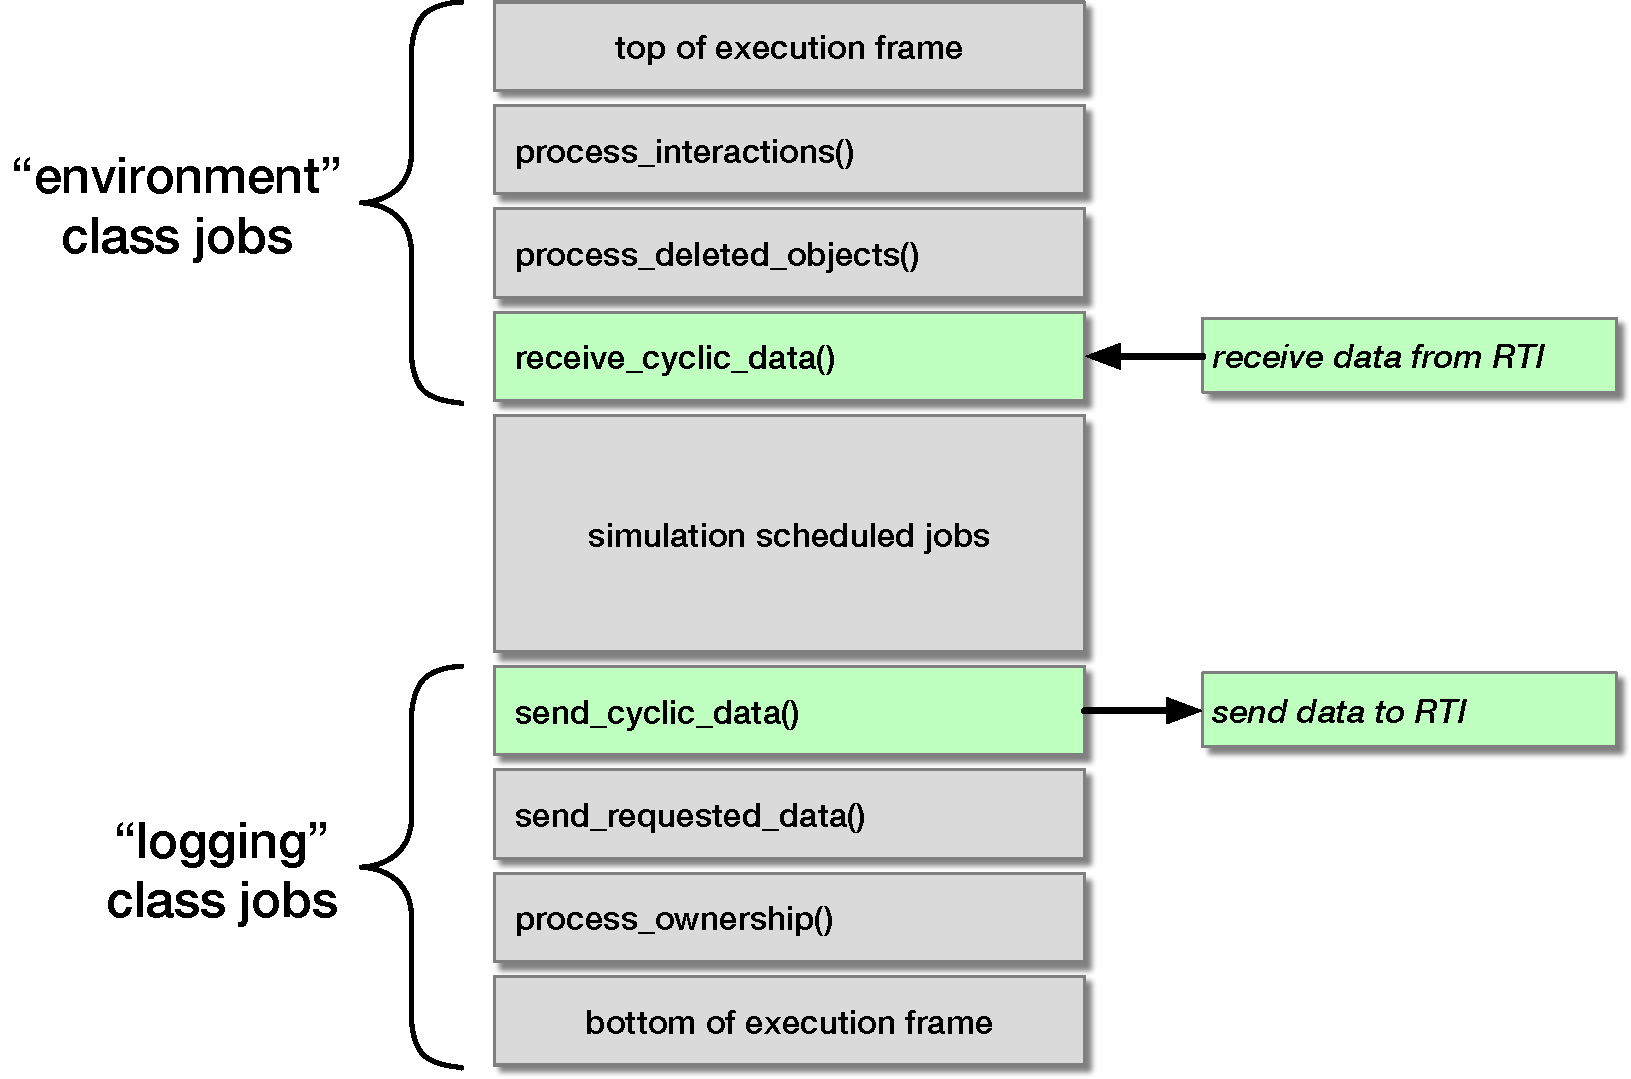
\includegraphics[scale=0.4]{TutorialTHLADataJobs.pdf}
      \end{figure}
   \end{frame}
   
   
   \section{Simulation Multiphase Initialization}

   \begin{frame}
      \frametitle{Simulation Multiphase Initialization}
      \begin{center}
      \Huge{Simulation Multiphase Initialization}
      \end{center}
   \end{frame}
   
   \begin{frame}[fragile]
      \frametitle{Simulation Multiphase Initialization}
      \begin{itemize}
         \item TrickHLA supports multiphase simulation initialization where data
         is exchanged between federates before the simulation starts running.
         \item An attribute is used for multiphase simulation initialization by
         specifying \texttt{THLA\_INITIALIZE} for the attribute’s config field
         (as in the previous example shown in the \texttt{RUN\_a\_side/input.py}
         file) :
\begin{Verbatim}[frame=single, fontsize=\scriptsize]
THLA.manager.objects[1].attributes[7].config = trick.THLA_INITIALIZE
                                               + trick.THLA_CYCLIC
\end{Verbatim}
      \end{itemize}
   \end{frame}
   
   \begin{frame}[fragile]
      \frametitle{Simulation Multiphase Initialization}
      \framesubtitle{\texttt{S\_define}: Public data and constructor}
      \begin{itemize}
         \item This is similar to our generic \texttt{THLA\_INIT} simulation object, but
         using a multiphase approach:
\begin{Verbatim}[frame=single, fontsize=\tiny]
. . .
// Include the simple simulation configuration object definition.
##include "simconfig/include/SimpleSimConfig.hh”
. . .

//=============================================================================
// SIM_OBJECT: THLA_INIT  (TrickHLA multi-phase initialization sim-object)
//=============================================================================
class THLAInitSimObj : public Trick::SimObject {

 public:

   TrickHLA::SimTimeline      sim_timeline;
   TrickHLA::ScenarioTimeline scenario_timeline;

   THLAInitSimObj( TrickHLA::Manager  & thla_mngr,
                   TrickHLA::Federate & thla_fed ) 
      : scenario_timeline( sim_timeline, 0.0, 0.0 ),
        thla_manager( thla_mngr ),
        thla_federate( thla_fed )
   {
\end{Verbatim}
      \end{itemize}
   \end{frame}
   
   \begin{frame}[fragile]
      \frametitle{Simulation Multiphase Initialization}
      \framesubtitle{\texttt{S\_define}: Public scheduled jobs}
      \begin{itemize}
         \item Declare the initialization jobs.
\begin{Verbatim}[frame=single, fontsize=\tiny]
      //------------------------------------------------------------------------
      // NOTE: Initialization phase numbers must be greater than P60 
      // (i.e. P_HLA_INIT) so that the initialization jobs run after the
      // P60 THLA.manager->initialize() job.
      //------------------------------------------------------------------------
      // Data will only be sent if this federate owns it.
      P100 ("initialization") thla_manager.send_init_data( "A-side-Federate.Test" );
      
      // Data will only be received if it is remotely owned by another federate.
      P100 ("initialization") thla_manager.receive_init_data( "A-side-Federate.Test" );
      
      // Do some processing here if needed...
      
      // Wait for all federates to reach this sync-point.
      P100 ("initialization") thla_manager.wait_for_init_sync_point( "Phase1" );
      
      // Data will only be sent if this federate owns it.
      P200 ("initialization") thla_manager.send_init_data( "P-side-Federate.Test" );
      
      // Data will only be received if it is remotely owned by another federate.
      P200 ("initialization") thla_manager.receive_init_data( "P-side-Federate.Test" );
      
      // Do some processing here if needed...
      
      // Wait for all federates to reach this sync-point.
      P200 ("initialization") thla_manager.wait_for_init_sync_point( "Phase2" );
   }
\end{Verbatim}
         \end{itemize}
   \end{frame}
   
   \begin{frame}[fragile]
      \frametitle{Simulation Multiphase Initialization}
      \framesubtitle{\texttt{S\_define}: Private data and instantiation}
      \begin{itemize}
         \item Protect from copies and do not permit a default constructor.
\begin{Verbatim}[frame=single, fontsize=\tiny]
      
 private:
   TrickHLA::Manager  & thla_manager;
   TrickHLA::Federate & thla_federate;
 
   // Do not allow the implicit copy constructor or assignment operator.
   THLAInitSimObj(const THLAInitSimObj & rhs);
   THLAInitSimObj & operator=(const THLAInitSimObj & rhs);
   
   // Do not allow the default constructor.
   THLAInitSimObj();
};
. . .
// Intantiate the initialization simulation object.
THLAInitSimObject THLA_INIT( THLA.manager, THLA.federate );
. . .
\end{Verbatim}
      \end {itemize}
   \end{frame}

   
      
   \section{Data Packing and Unpacking}

   \begin{frame}
      \frametitle{Data Packing and Unpacking}
      \begin{center}
      \Huge{Data Packing and Unpacking}
      \end{center}
   \end{frame}
   
   \begin{frame}
      \frametitle{Data Packing and Unpacking}
      \begin{itemize}
         \item TrickHLA supports a data packing and unpacking mechanism so that
         data transformations can be applied to the data before being sent to
         (pack) or after received from (unpack) another federate.
         \item For example, your simulation uses a phase variable in radians but
         the FOM specifies the phase variable  will be exchanged between
         federates in degrees.
         \item Packing/unpacking is added to your simulation by extending the
         \texttt{TrickHLAPacking} class and implementing the \texttt{pack()}
         and \texttt{unpack()} functions.
         \item TrickHLA will automatically call your \texttt{pack()} and
         \texttt{unpack()}
         functions at the appropriate time.
         \item Adding packing/unpacking to your simulation consists of three
         steps \textellipsis
      \end{itemize}
   \end{frame}

   \begin{frame}[fragile]
      \frametitle{Data Packing and Unpacking}
      \framesubtitle{Step 1: Extending the \texttt{TrickHLA::Packing} Class - \texttt{SinePacking.hh}}
      \begin{itemize}
         \item Step 1: Extend the \texttt{TrickHLA::Packing} class and implement
         the \texttt{pack()} and \texttt{unpack()} functions in \texttt{SinePacking.hh} :
      \end{itemize}
\begin{Verbatim}[frame=single, fontsize=\tiny]
   #include SineData.hh
   #include "TrickHLA/include/TrickHLAPacking.hh"

   class SinePacking : public TrickHLAPacking
   {
     public:
      // Initialize the packing object.
      void initialize( SineData * sim_data );
      // From the TrickHLAPacking class.
      virtual void initialize_callback( TrickHLAObject * obj );

      // From the TrickHLAPacking class.
      virtual void pack();
      // From the TrickHLAPacking class.
      virtual void unpack();

     private:
      SineData * sim_data; // -- Simulation data.
      double phase_deg;    // d  Phase offset in degrees.
   };
\end{Verbatim}
   \end{frame}

   \begin{frame}[fragile]
      \frametitle{Data Packing and Unpacking}
      \framesubtitle{Step 1: Extending the \texttt{TrickHLA::Packing} Class - \texttt{SinePacking.cpp}}
      \begin{itemize}
         \item Example in \texttt{SinePacking.cpp} :
      \end{itemize}
\begin{Verbatim}[frame=single, fontsize=\scriptsize]
void SinePacking::initialize( // RETURN: -- None.
      SineData * sim_data)    // IN:     -- Simulation data.
{
   this->sim_data = sim_data;
}
void SinePacking::pack()    // RETURN: -- None.
{
   // For this example to show how to use the Packing API's, we
   // will assume that the phase shared between federates is in
   // degrees so convert it from radians to degrees.
   phase_deg = sim_data->get_phase() * 180.0 / M_PI;
}
void SinePacking::unpack()  // RETURN: -- None.
{
   // For this example to show how to use the Packing API's, we
   // will assume that the phase shared between federates is in
   // degrees so convert it back from degrees to radians.
   sim_data->set_phase( phase_deg * M_PI / 180.0 );
}
\end{Verbatim}
   \end{frame}

   \begin{frame}[fragile]
      \frametitle{Data Packing and Unpacking}
      \framesubtitle{Step 2: Add Packing Object to \texttt{S\_define}}
      \begin{itemize}
         \item Step 2: In the \texttt{S\_define} file add your packing object
         to each simulation object that needs to have its data packed/unpacked.
         \item Make sure to initialize your packing object if it needs it.
      \end{itemize}
\begin{Verbatim}[frame=single, fontsize=\tiny]
   class ASimObject : public Trick::SimObject {
      …
      SineData     sim_data;
      SinePacking  packing;

      ASimObject() {
        P50 ("initialization") packing.initialize( &sim_data );
        …
      }
   };

   class PSimObject : public Trick::SimObject {
      …
      SineData     sim_data;
      SinePacking  packing;

      PSimObject() {
        P50 ("initialization") packing.initialize( &sim_data );
        …
      }
   };
\end{Verbatim}
   \end{frame}

   \begin{frame}[fragile]
      \frametitle{Data Packing and Unpacking}
      \framesubtitle{Step 3: Configuration}
      \begin{itemize}
         \item Step 3: Configure the data object in the input.py file to use
         your packing object by setting the data object’s packing field. For
         example in the \texttt{RUN\_a\_side/input.py} file:
\begin{Verbatim}[frame=single, fontsize=\scriptsize]
THLA.manager.objects[0].packing = A.packing
THLA.manager.objects[1].packing = P.packing
\end{Verbatim}
         \item Don’t forget to update the attribute \texttt{trick\_name} field
         to use the correct Trick simulation variable (i.e. the transformed
         data from the \texttt{pack()} and \texttt{unpack()} functions).
   To use the simulation data phase in radians:
\begin{Verbatim}[frame=single, fontsize=\scriptsize]
THLA.manager.objects[0].attributes[3].trick_name = "A.sim_data.phase”
THLA.manager.objects[1].attributes[3].trick_name = “P.sim_data.phase”
\end{Verbatim}
         \item To use the transformed phase in degrees to be shared with the
         other federates:
\begin{Verbatim}[frame=single, fontsize=\scriptsize]
THLA.manager.objects[0].attributes[3].trick_name = "A.packing.phase_deg”
THLA.manager.objects[1].attributes[3].trick_name = “P.packing.phase_deg”
\end{Verbatim}
      \end{itemize}
   \end{frame}

   \begin{frame}
      \frametitle{Data Packing and Unpacking}
      \framesubtitle{TrickHLA jobs in THLA.sm}
      \begin{figure}
      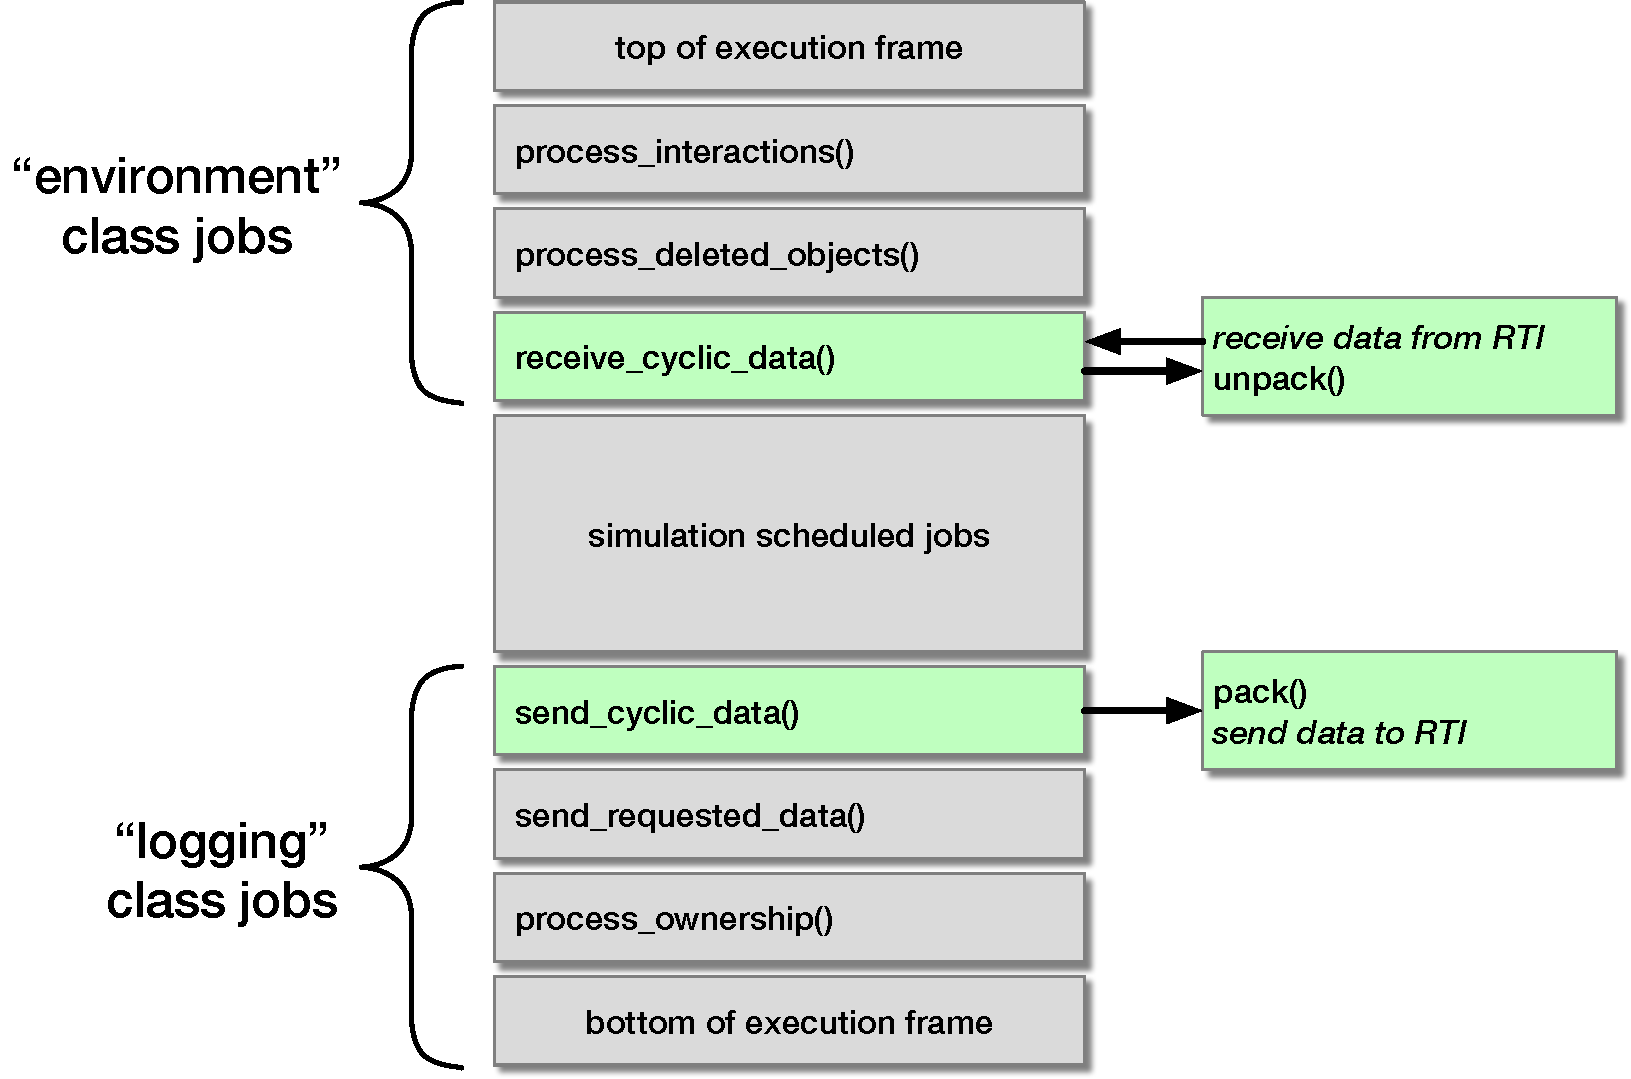
\includegraphics[scale=0.4]{TutorialTHLAPackingJobs.pdf}
      \end{figure}
   \end{frame}
   
      
   \section{Interactions}

   \begin{frame}
      \frametitle{Interactions}
      \begin{center}
      \Huge{Interactions}
      \end{center}
   \end{frame}
   
   \begin{frame}
      \frametitle{Interactions}
      \begin{itemize}
         \item TrickHLA supports interactions that are either Timestamp Order
         (TSO) or Receive Order (RO).
         \item Configuring TrickHLA interactions involves three steps:
         \begin{itemize}
            \item Step 1: Extend the \texttt{TrickHLA::InteractionHandler} class
            and implement the virtual \texttt{receive\_interaction()} function.
            \item Step 2: Add your interaction-handler object to each simulation
            object that needs to process interactions in your \texttt{S\_define} file.
            \item Step 3: Configure the interaction-handlers in the \texttt{input.py} file.
            \item Step 4: Send interactions at specified times using the
            \texttt{input.py} file or programmatically within your simulation.
         \end{itemize}
      \end{itemize}
   \end{frame}
   
   \begin{frame}[fragile]
      \frametitle{Interactions}
      \framesubtitle{Step 1: Extend the \texttt{TrickHLA::InteractionHandler} Class}
      \begin{itemize}
         \item Step 1: This is a snippet of the base class from
         \texttt{TrickHLA::InteractionHandler.hh} that you must extend and then
         implement the virtual \texttt{receive\_interaction()} function:
      \end{itemize}
\begin{Verbatim}[frame=single, fontsize=\scriptsize]
class TrickHLA::InteractionHandler
{
  ...
  public:
   ...
   virtual void initialize_callback( TrickHLAInteraction * inter );

   bool send_interaction();                   // Receive Order
   bool send_interaction( double send_time ); // Timestamp Order

   // This is a virtual function and must be defined by a full class.
   virtual void receive_interaction();
   ...
};
\end{Verbatim}
   \end{frame}

   \begin{frame}[fragile]
      \frametitle{Interactions}
      \framesubtitle{Step 1: Extend the \texttt{TrickHLA::InteractionHandler} - \texttt{SineInteractionHandler.hh}}
      \begin{itemize}
         \item Extended in \texttt{SineInteractionHandler.hh}:
      \end{itemize}
      \vspace{0.2cm}
\begin{Verbatim}[frame=single, fontsize=\tiny]
#include "TrickHLA/include/TrickHLAInteractionHandler.hh"

class SineInteractionHandler : public TrickHLAInteractionHandler
{
  ...
  public:
   ...
   void send_sine_interaction( double sim_time );

   virtual void receive_interaction();

   char *   name;    // -- Example of a unique name to identify the interaction handler.
   char *   message; // -- Example of a static array of strings.

  protected:
   double   time;        // s  Example of floating-point data.
   int      year;        // -- Example of integer data.
   int      send_cnt;    // -- The number of times an interaction is sent.
   int      receive_cnt; // -- The number of times an interaction was received.};
};
\end{Verbatim}
   \end{frame}

   \begin{frame}[fragile]
      \frametitle{Interactions}
      \framesubtitle{Step 1: Extend the \texttt{TrickHLA::InteractionHandler} - \texttt{SineInteractionHandler.cpp}}
      \begin{itemize}
         \item Extended in \texttt{SineInteractionHandler.cpp}:
      \end{itemize}
\begin{Verbatim}[frame=single, fontsize=\tiny]
void SineInteractionHandler::send_sine_interaction( // RETURN: -- None.
   double sim_time)        // IN: s Current simulation time.
{
   time = sim_time;    // Update the time with the simulation time.
   ostringstream msg;  // Create a message to send
   msg << "Interaction from:\"" << ((name != NULL) ? name : "Unknown") << "\" "
       << "Send-count:" << (send_cnt + 1);
   if ( ( message != NULL ) && TMM_is_alloced( message ) ) {
      TMM_delete_var_a( message );
   }
   message = TMM_strdup( (char *)msg.str().c_str() );

   double lookahead_time = get_fed_lookahead().getDoubleTime();
   double timestamp = time + lookahead_time;
   // Notify the parent interaction handler to send the interaction using
   // Timestamp Order (TSO) at the current simulation time plus the lookahead_time.
   bool was_sent = this->TrickHLAInteractionHandler::send_interaction( timestamp );
   if ( was_sent ) {
      cout << "++++SENDING++++ SineInteractionHandler::send_sine_interaction() << endl
           << "  name:'" << ((name != NULL) ? name : "NULL") << "'" << endl
           << "  message:'" << ((message != NULL) ? message : "NULL") << "'" << endl
           << "  timestamp:" << timestamp;
      send_cnt++; // Update send count, just used for the message in this example
   } else {
      cout << "+-+-NOT SENT-+-+ SineInteractionHandler::send_sine_interaction()" << endl         
}
\end{Verbatim}
   \end{frame}

   \begin{frame}[fragile]
      \frametitle{Interactions}
      \framesubtitle{Step 1: Extend the \texttt{TrickHLA::InteractionHandler} - \texttt{SineInteractionHandler.cpp}}
      \begin{itemize}
         \item Extended in \texttt{SineInteractionHandler.cpp} (Continued):
      \end{itemize}
      \vspace{0.2cm}
\begin{Verbatim}[frame=single, fontsize=\tiny]
void SineInteractionHandler::receive_interaction() // RETURN: -- None.
{
   receive_cnt++;
   double sim_time = exec_get_sim_time();

   cout << "++++RECEIVING++++ SineInteractionHandler::receive_interaction()" << endl
        << "  name:'" << ((name != NULL) ? name : "NULL") << "'" << endl
        << "  message:'" << ((message != NULL) ? message : "NULL") << "'" << endl
        << "  message length:" << ((message != NULL) ? strlen(message) : 0) << endl
        << "  sim_time:" << sim_time << endl
        << "  time:" << time << endl
        << "  year:" << year << endl
        << "  receive_cnt:" << receive_cnt << endl;
}
\end{Verbatim}
   \end{frame}

   \begin{frame}[fragile]
      \frametitle{Interactions}
      \framesubtitle{Step 2: Add Interaction-handler Object to \texttt{S\_define}}
      \begin{itemize}
         \item Step 2: In the \texttt{S\_define} file add your interaction-handler
         object to each simulation object that needs to process interactions.  
      \end{itemize}
\begin{Verbatim}[frame=single, fontsize=\tiny]
   class ASimObject : public Trick::SimObject {

      SineData     sim_data;
      SinePacking            packing;
      SineInteractionHandler interaction_handler;

      ASimObject() {
        P50 ("initialization") packing.initialize( &sim_data );
        ...
      }
   };

   class PSimObject : public Trick::SimObject {
      ...
      SineData     sim_data;
      SinePacking            packing;
      SineInteractionHandler interaction_handler;

      PSimObject() {
        P50 ("initialization") packing.initialize( &sim_data );
        ...
      }
   };
\end{Verbatim}
   \end{frame}

   \begin{frame}[fragile]
      \frametitle{Interactions}
      \framesubtitle{Step 3: Configure the interaction-handlers in the \texttt{input.py} file}
      \begin{itemize}
         \item Step 3: Example in the \texttt{RUN\_a\_side/input.py} file:
      \end{itemize}
\begin{Verbatim}[frame=single, fontsize=\tiny]
# We are taking advantage of the input file to specify a unique name for each handler
A.interaction_handler.name = "A-side: A.interaction_handler.name"
P.interaction_handler.name = "A-side: P.interaction_handler.name"

# Trick HLA Interactions and Parameters.
THLA.manager.inter_count  = 1
THLA.manager.interactions = trick.alloc_type( THLA.manager.inter_count, "TrickHLAInteraction" )

THLA.manager.interactions[0].FOM_name    = "Communication"
THLA.manager.interactions[0].publish     = True
THLA.manager.interactions[0].subscribe   = False
THLA.manager.interactions[0].handler     = A.interaction_handler
THLA.manager.interactions[0].param_count = 3
THLA.manager.interactions[0].parameters  = trick.alloc_type( THLA.manager.interactions[0].param_count,
                                           "TrickHLAParameter" )
THLA.manager.interactions[0].parameters[0].FOM_name   = "Message"
THLA.manager.interactions[0].parameters[0].trick_name = "A.interaction_handler.message"
THLA.manager.interactions[0].parameters[0].rti_encoding = trick.THLA_UNICODE_STRING

THLA.manager.interactions[0].parameters[1].FOM_name   = "time"
THLA.manager.interactions[0].parameters[1].trick_name = "A.interaction_handler.time"
THLA.manager.interactions[0].parameters[1].rti_encoding = trick.THLA_LITTLE_ENDIAN

THLA.manager.interactions[0].parameters[2].FOM_name   = "year"
THLA.manager.interactions[0].parameters[2].trick_name = "A.interaction_handler.year"
THLA.manager.interactions[0].parameters[2].rti_encoding = trick.THLA_LITTLE_ENDIAN
\end{Verbatim}
   \end{frame}

   \begin{frame}[fragile]
      \frametitle{Interactions}
      \framesubtitle{Step 3: Configure the interaction-handlers in the \texttt{input.py} file}
      \begin{itemize}
         \item Step 3: Example in the \texttt{RUN\_p\_side/input.py} file:
      \end{itemize}
\begin{Verbatim}[frame=single, fontsize=\tiny]
# We are taking advantage of the input file to specify a unique name for each handler
A.interaction_handler.name = P-side: A.interaction_handler.name"
P.interaction_handler.name = P-side: P.interaction_handler.name"

# TrickHLA Interactions and Parameters.
THLA.manager.inter_count  = 1
THLA.manager.interactions = trick.alloc_type( THLA.manager.inter_count, "TrickHLAInteraction" )

THLA.manager.interactions[0].FOM_name    = "Communication"
THLA.manager.interactions[0].publish     = False
THLA.manager.interactions[0].subscribe   = True
THLA.manager.interactions[0].handler     = P.interaction_handler
THLA.manager.interactions[0].param_count = 3
THLA.manager.interactions[0].parameters  = trick.alloc_type( THLA.manager.interactions[0].param_count,
                                           "TrickHLAParameter" )
THLA.manager.interactions[0].parameters[0].FOM_name   = "Message"
THLA.manager.interactions[0].parameters[0].trick_name = "P.interaction_handler.message"
THLA.manager.interactions[0].parameters[0].rti_encoding = trick.THLA_UNICODE_STRING

THLA.manager.interactions[0].parameters[1].FOM_name   = "time"
THLA.manager.interactions[0].parameters[1].trick_name = "P.interaction_handler.time"
THLA.manager.interactions[0].parameters[1].rti_encoding = trick.THLA_LITTLE_ENDIAN

THLA.manager.interactions[0].parameters[2].FOM_name   = "year"
THLA.manager.interactions[0].parameters[2].trick_name = "P.interaction_handler.year"
THLA.manager.interactions[0].parameters[2].rti_encoding = trick.THLA_LITTLE_ENDIAN
\end{Verbatim}
   \end{frame}

   \begin{frame}[fragile]
      \frametitle{Interactions}
      \framesubtitle{Step 4: Sending Interactions Using the Input File}
      \begin{itemize}
         \item Step 4: Add entries to the \texttt{input.py} file for when you
         want to send an interaction. For example, to send an interaction at
         time 10.0:
      \vspace{0.2cm}
\begin{Verbatim}[frame=single, fontsize=\tiny]
trick.add_read( 10.0, A.interaction_handler.send_sine_interaction(10.0) )
\end{Verbatim}
      \end{itemize}
   \end{frame}

   \begin{frame}
      \frametitle{Interactions}
      \framesubtitle{Sending and Receiving Interactions}
      \begin{itemize}
         \item Sending an interaction can be initiated three different ways:
         \begin{itemize}
            \item Programmatically, call one of the \texttt{send\_interaction()}
            functions inherited by your interaction-handler.
            \item As a job in your simulation specified in the \texttt{S\_define}
            file, which in turn calls \texttt{send\_interaction()} as above.
            \item As a job in your simulation called at a specific time from the
            \texttt{input.py} file, which in turn calls \texttt{send\_interaction()}
            as above.
         \end{itemize}
         \item TrickHLA will automatically process received interactions and
         call the \texttt{receive\_interaction()} function of the appropriate
         user defined interaction-handler.
         \item TrickHLA handles interactions in a thread-safe and Trick
         simulation environment job-safe way.
      \end{itemize}
   \end{frame}

   \begin{frame}
      \frametitle{Interactions}
      \framesubtitle{TrickHLA jobs in THLA.sm}
      \begin{figure}
      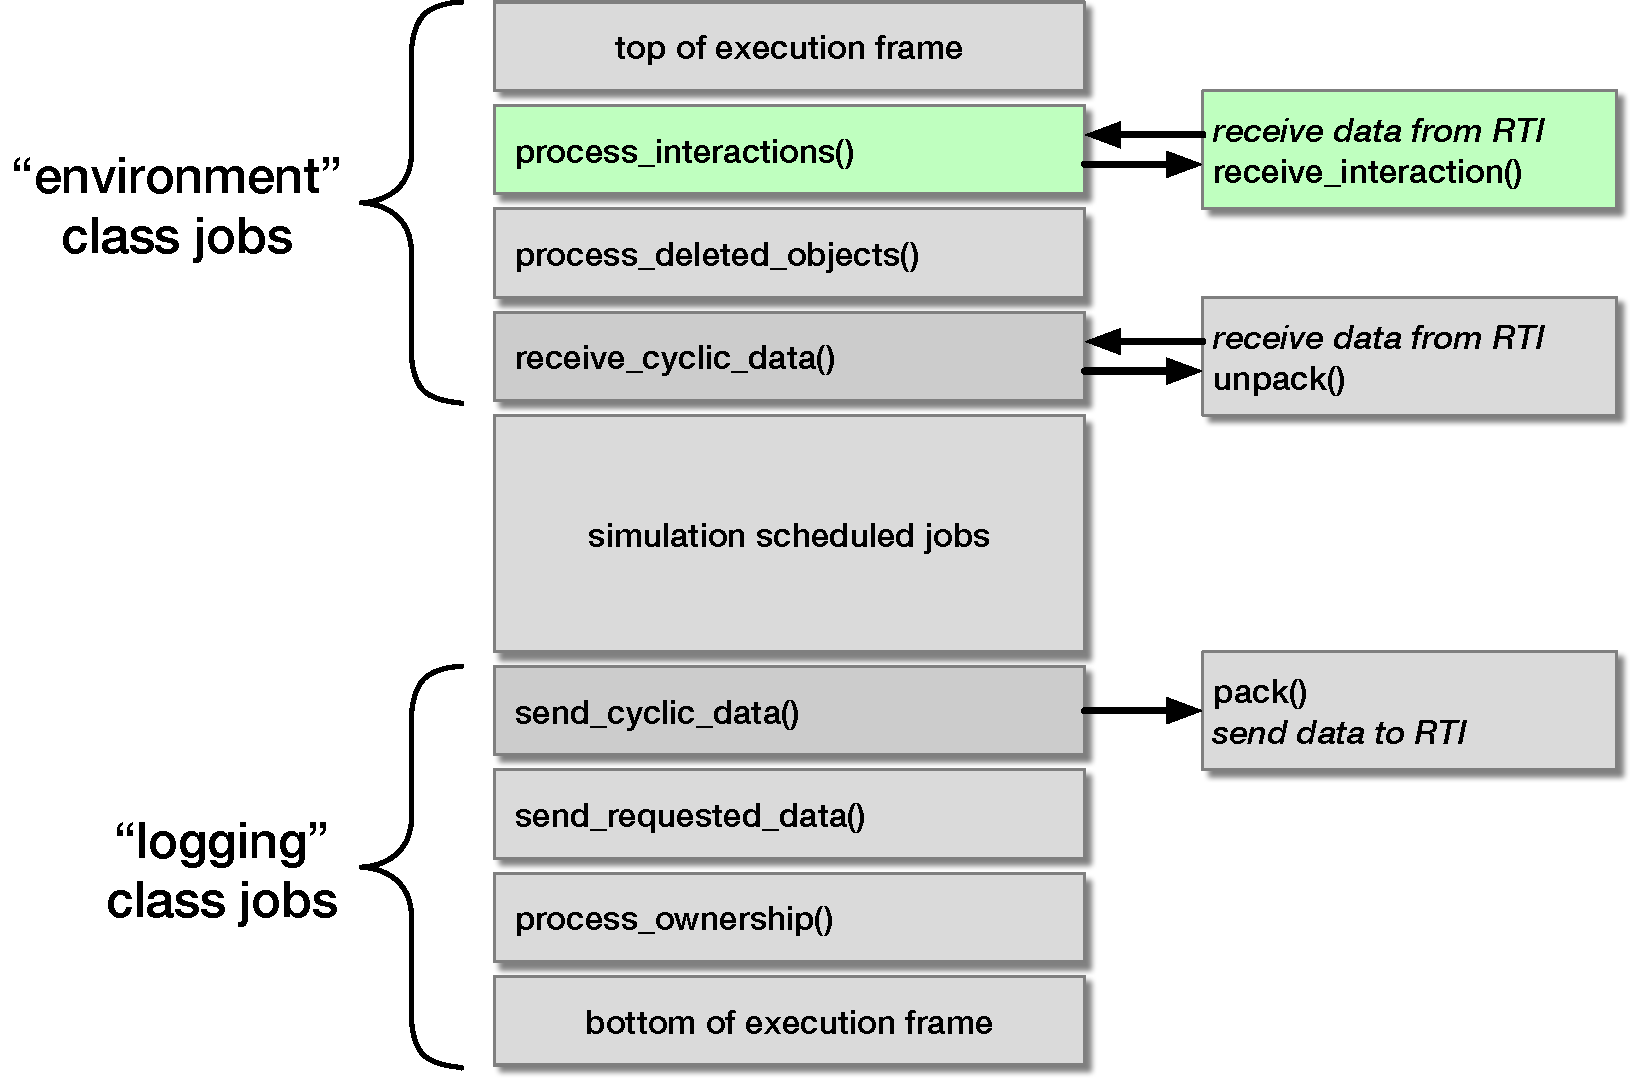
\includegraphics[scale=0.4]{TutorialTHLAInteractionJobs.pdf}
      \end{figure}
   \end{frame}
   

   
   
   \section{Lag Compensation}

   \begin{frame}
      \frametitle{Lag Compensation}
      \begin{center}
      \Huge{Lag Compensation}
      \end{center}
   \end{frame}
   
   \begin{frame}
      \frametitle{Lag Compensation}
      \begin{itemize}
         \item An in depth discussion of lag/latency compensation goes beyond
         the scope of this training.  Please see the following paper for more
         detailed information on the subject:
      \end{itemize}
         \begin{scriptsize}
         \begin{quote}
         \textit{R. Phillips, E. Crues, Time Management Issues and Approaches
         for Real Time HLA Based Simulations, Proceedings of the Fall 2005
         Simulation Interoperability Workshop and Conference, Fall 2005.}
         \end{quote}
         \end{scriptsize}
      \begin{itemize}
         \item Lag Compensation is an attempt to correct for the time difference
         between when a state is published at one federate and received at
         another federate.
         \item Using TrickHLA lag compensation consists of four steps:
         \begin{itemize}
            \item Step 1: Extend the \texttt{TrickHLALagCompensation} class and
            implement the \texttt{sending\_lag\_compensation()} and
            \texttt{receive\_lag\_compensation()} virtual functions.
            \item Step 2: In the \texttt{S\_define} file add a lag-compensation
            object to each simulation object that needs to perform lag compensation.
            \item Step 3: Configure lag compensation in the \texttt{input.py} file.
            \item Step 4: Update the object attributes in the \texttt{input.py}
            file to use the lag compensated Trick simulation variable.
         \end{itemize}
      \end{itemize}
   \end{frame}

   \begin{frame}[fragile]
      \frametitle{Lag Compensation}
      \framesubtitle{Step 1: Extend the \texttt{TrickHLALagCompensation} Class}
      \begin{itemize}
         \item Step 1: Extend the \texttt{TrickHLALagCompensation} class and
         implement the \texttt{sending\_lag\_compensation()} and
         \texttt{receive\_lag\_compensation()} virtual functions. Example in
         \texttt{SineLagCompensation.hh}:
      \vspace{0.2cm}
\begin{Verbatim}[frame=single, fontsize=\tiny]
#include "SineData.hh"
#include "TrickHLA/include/TrickHLALagCompensation.hh"

class SineLagCompensation : public TrickHLALagCompensation
{
...
public:
   // From the TrickHLALagCompensation class.
   virtual void sending_lag_compensation( double current_time, double dt );

   // From the TrickHLALagCompensation class.
   virtual void receive_lag_compensation( double current_time, double dt );
...
};
\end{Verbatim}
         \item TrickHLA will automatically call the send or receive lag
         compensation functions at the appropriate time.
      \end{itemize}
   \end{frame}

   \begin{frame}[fragile]
      \frametitle{Lag Compensation}
      \framesubtitle{Step 2: Add Lag-compensation Object to \texttt{S\_define}}
      \begin{itemize}
         \item Step 2: In the \texttt{S\_define} file add a lag-compensation
         object to each simulation object that needs to perform lag compensation.
         Make sure to initialize your lag-compensation object if it needs it.
      \end{itemize}
\begin{Verbatim}[frame=single, fontsize=\scriptsize]
   class ASimObject : public Trick::SimObject {
      ...
      SineData     sim_data;
      SineData     lag_comp_data;
      SinePacking            packing;
      SineLagCompensation    lag_compensation;
      SineInteractionHandler interaction_handler;

      ASimObject() {
        P50 ("initialization") packing.initialize( &sim_data );
        P50 ("initialization") lag_compensation.initialize( &sim_data, 
                                                            &lag_comp_data );
        ...
      }
   };
\end{Verbatim}
   \end{frame}

   \begin{frame}[fragile]
      \frametitle{Lag Compensation}
      \framesubtitle{Step 3: Configuration}
      \begin{itemize}
         \item Step 3: Configure lag compensation in the \texttt{input.py} file.
         \vspace{0.2cm}
\begin{Verbatim}[frame=single, fontsize=\scriptsize]
THLA.manager.objects[0].lag_comp      = A.lag_compensation
THLA.manager.objects[0].lag_comp_type = trick.THLA_LAG_COMP_SENDING
\end{Verbatim}
      \item The supported lag compensation types are:
         \begin{itemize}
            \item \texttt{THLA\_LAG\_COMP\_NONE}  (default)
            \item \texttt{THLA\_LAG\_COMP\_SENDING}
            \item \texttt{THLA\_LAG\_COMP\_RECEIVE}
         \end{itemize}
      \end{itemize}
   \end{frame}

   \begin{frame}[fragile]
      \frametitle{Lag Compensation}
      \framesubtitle{Step 4: Update Object Attributes}
      \begin{itemize}
         \item Step 4: Update the attribute \texttt{trick\_name} field in the
         \texttt{input.py} file to use the lag compensated Trick simulation variable.
         \item If the lag compensation type is \texttt{THLA\_LAG\_COMP\_NONE}:
         \vspace{0.2cm}
\begin{Verbatim}[frame=single, fontsize=\scriptsize]
THLA.manager.objects[0].attributes[1].FOM_name   = "Value"
THLA.manager.objects[0].attributes[1].trick_name = "A.sim_data.value"
\end{Verbatim}
      \item If the lag compensation type is \texttt{THLA\_LAG\_COMP\_SENDING}
      or \texttt{THLA\_LAG\_COMP\_RECEIVE}:
         \vspace{0.2cm}
\begin{Verbatim}[frame=single, fontsize=\scriptsize]
THLA.manager.objects[0].attributes[1].FOM_name   = "Value"
THLA.manager.objects[0].attributes[1].trick_name = "A.lag_comp_data.value"
\end{Verbatim}
      \end{itemize}
   \end{frame}

   \begin{frame}
      \frametitle{Lag Compensation}
      \framesubtitle{Combinations}
      \begin{itemize}
         \item The five logical combinations of lag compensation between two
         federates is shown in the table below:
      \end{itemize}
\begin{tiny}
\begin{center}
\begin{tabular}{|l|l|l|} \hline
\textbf{Lag Comp. Type} & \textbf{A-side-Federate} & \textbf{P-side-Federate} \\ \hline
None & Publish: THLA\_LAG\_COMP\_NONE   & Subscribe: THLA\_LAG\_COMP\_NONE \\
     & Subscribe: THLA\_LAG\_COMP\_NONE & Publish: THLA\_LAG\_COMP\_NONE \\ \hline
Sending-side & Publish: THLA\_LAG\_COMP\_SENDING & Subscribe: THLA\_LAG\_COMP\_NONE \\
             & Publish: THLA\_LAG\_COMP\_SENDING & Subscribe: THLA\_LAG\_COMP\_NONE \\ \hline
Receive-side & Publish: THLA\_LAG\_COMP\_NONE & Subscribe: THLA\_LAG\_COMP\_RECEIVE \\
             & Publish: THLA\_LAG\_COMP\_NONE & Subscribe: THLA\_LAG\_COMP\_RECEIVE \\ \hline
Sending- and & Publish: THLA\_LAG\_COMP\_SENDING & Subscribe: THLA\_LAG\_COMP\_RECEIVE \\
Receive-side & Subscribe: THLA\_LAG\_COMP\_NONE  & Publish: THLA\_LAG\_COMP\_NONE \\ \hline
Sending- and & Publish: THLA\_LAG\_COMP\_NONE    & Subscribe: THLA\_LAG\_COMP\_NONE \\
Receive-side & Publish: THLA\_LAG\_COMP\_SENDING & Subscribe: THLA\_LAG\_COMP\_RECEIVE \\ \hline
\end{tabular}
\end{center}
\end{tiny}
      \begin{itemize}
         \item "Publish" refers to the attributes the federate is configured to
         send data for.
         \item "Subscribe" refers to the attributes the federate is configured
         to receive data for.
      \end{itemize}
   \end{frame}

   \begin{frame}
      \frametitle{Lag Compensation}
      \framesubtitle{TrickHLA jobs in THLA.sm}
      \begin{figure}
      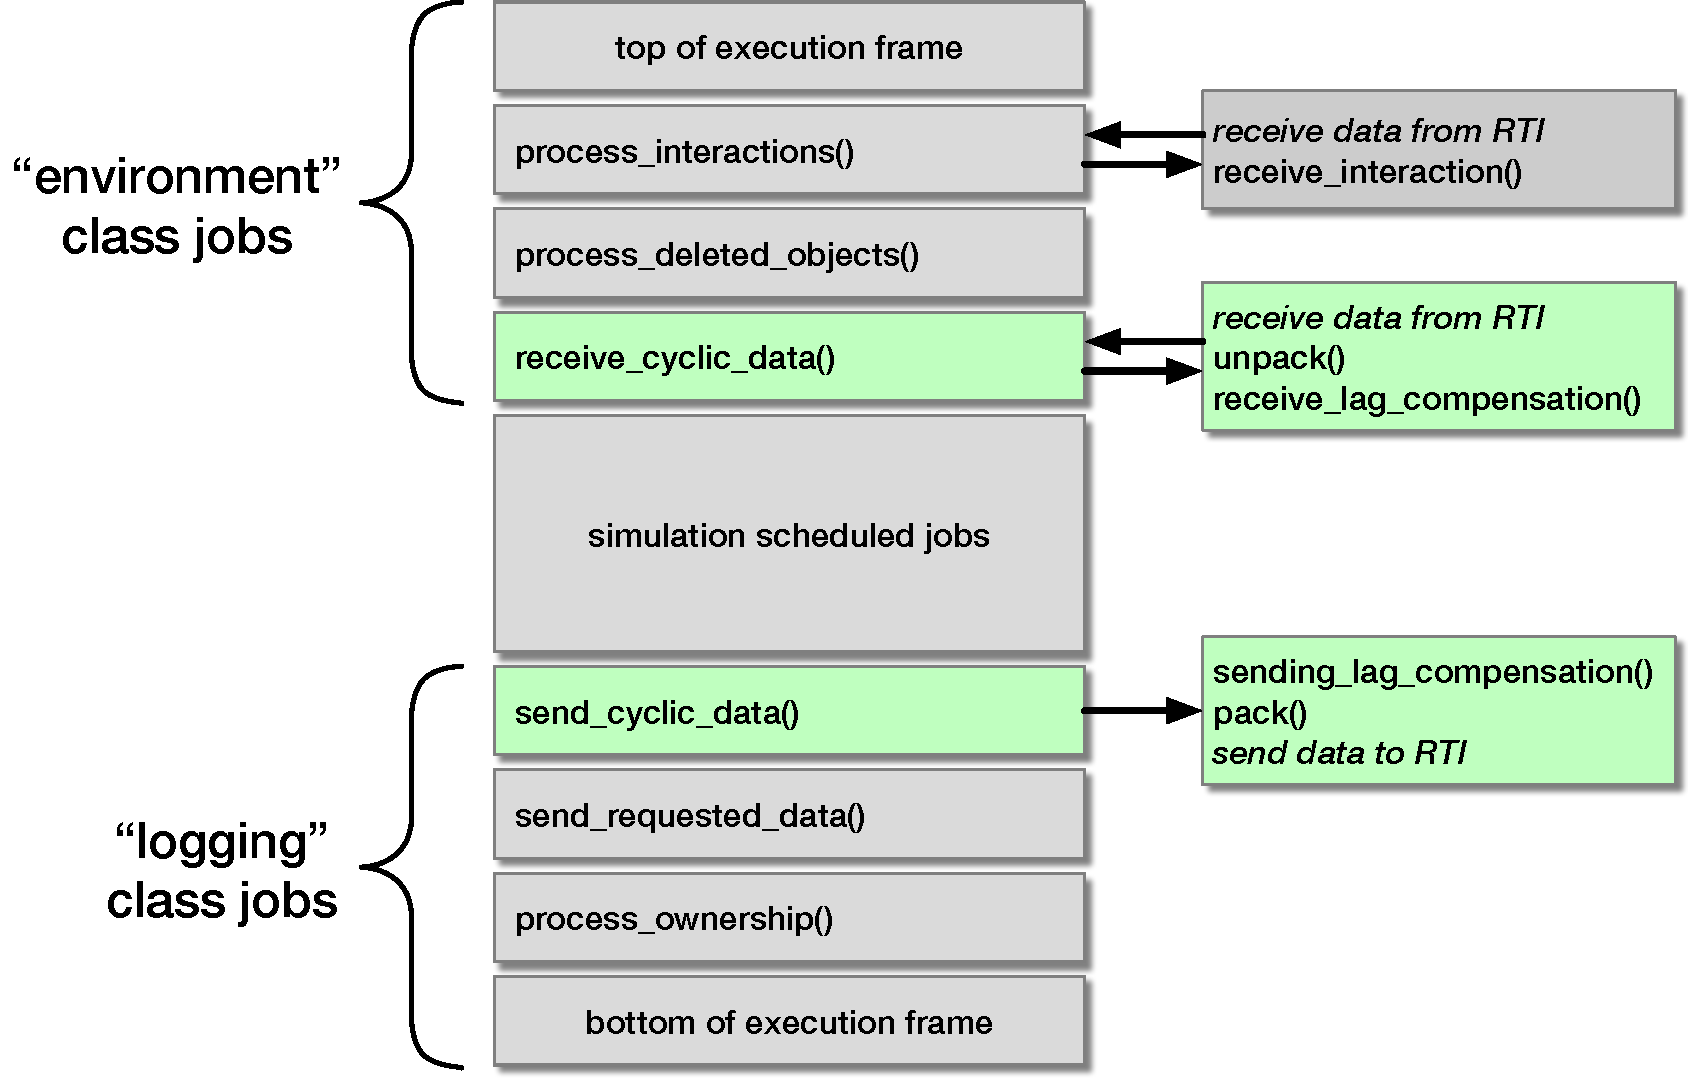
\includegraphics[scale=0.4]{TutorialTHLALagCompJobs.pdf}
      \end{figure}
   \end{frame}


   
   
   \section{Ownership Transfer}

   \begin{frame}
      \frametitle{Ownership Transfer}
      \begin{center}
      \Huge{Ownership Transfer}
      \end{center}
   \end{frame}
   
   \begin{frame}
      \frametitle{Ownership Transfer}
      \begin{small}
      \begin{itemize}
         \item TrickHLA supports ownership transfer down to the individual attribute.
         \item Ownership of attributes can be Pulled from the owning federate or federates.
         \item Ownership of attributes can be Pushed to any accepting federate or federates.
         \item Multiple Push/Pull requests can be scheduled for different times
         and for specific attributes or all attributes.
         \item Automatically handles attribute state publication until attribute
         ownership has been transferred.
         \item Pushing attribute ownership will result in the RTI deciding which
         federate(s) get ownership of which attributes. You don’t have control
         over which federate you get to push attribute ownership to.
         \item Pulling attribute ownership gives you control over which federate
         gets ownership of a particular attribute.
         \item There are two approaches to using ownership transfer:
         \begin{itemize}
            \item Programmatically, which requires more programming effort.
            \item Entries in the \texttt{input.py} file, which requires the least effort.
         \end{itemize}
      \end{itemize}
      \end{small}
   \end{frame}

   \begin{frame}[fragile]
      \frametitle{Ownership Transfer}
      \framesubtitle{Attribute Publish, Subscribe, and Locally\_Owned Fields}
      \begin{itemize}
         \item The state of the publish, subscribe and locally\_owned attribute
         fields (in the \texttt{input.py} file) affect ownership transfer.
         \vspace{0.2cm}
\begin{Verbatim}[frame=single, fontsize=\footnotesize]
THLA.manager.objects[0].attributes[1].publish       = True
THLA.manager.objects[0].attributes[1].subscribe     = True
THLA.manager.objects[0].attributes[1].locally_owned = True
\end{Verbatim}
      \end{itemize}
\begin{tiny}
\begin{center}
\begin{tabular}{|c|c|C{1.7cm}|C{1.7cm}|C{1.7cm}|C{1.7cm}|} \hline
\textbf{Pulish} & \textbf{Locally Owned} & \textbf{Push Ownership to Another Federate}
& \textbf{Pull Ownership from Another Federate}
& \textbf{Another Federate Wants to Pull Ownership}
& \textbf{Another Federate Wants to Push Ownership} \\ \hline
True  & True  & Yes & No  & Yes & No  \\ \hline
True  & False & No  & Yes & No  & Yes \\ \hline
False & True  & Yes & No  & Yes & No  \\ \hline
False & False & No  & No  & No  & No  \\ \hline
\end{tabular}
\end{center}
\end{tiny}
\begin{scriptsize}
\begin{center}
\begin{tabular}{|c|C{5cm}|} \hline
\textbf{Subscribe} & \textbf{Will receive attribute reflections \newline when locally\_owned == false?} \\ \hline
True & Yes \\ \hline
False & No \\ \hline
\end{tabular}
\end{center}
\end{scriptsize}
   \end{frame}

   \begin{frame}
      \frametitle{Ownership Transfer}
      \framesubtitle{Configuration}
      \begin{itemize}
         \item The approach of programmatically performing ownership transfers
         requires more programming effort and has three steps:
         \begin{itemize}
            \item Step 1: Extend the \texttt{TrickHLAOwnershipHandler} class.
            \item Step 2: In the \texttt{S\_define} file add your ownership-handler to
            each simulation object that needs to process ownership transfers.
            \item Step 3: Configure ownership transfer in the \texttt{input.py} file.
         \end{itemize}
         \item The approach of using the input.py file for ownership transfer
         requires the least effort and has three steps:
         \begin{itemize}
            \item Step 1: In the \texttt{S\_define} file add the default ownership-handler
            to each simulation object that needs to process ownership transfers.
            \item Step 2: Configure ownership transfer in the input.py file.
            \item Step 3: Add entries to the \texttt{input.py} file for when you
            want to push or pull ownership.
         \end{itemize}
      \end{itemize}
   \end{frame}

   \begin{frame}[fragile]
      \frametitle{Ownership Transfer}
      \framesubtitle{Programmatic Approach – Step 1}
      \begin{itemize}
         \item Step 1: This is a snippet of the base class from
         \texttt{TrickHLAOwnershipHandler.hh} that you must extend. 
      \end{itemize}
\begin{Verbatim}[frame=single, fontsize=\Tiny]
class TrickHLAOwnershipHandler
{
   ...
  public:
   virtual void initialize_callback( TrickHLAObject * obj );

   string get_object_name();
   string get_object_FOM_name();

   int get_attribute_count();
   VectorOfStrings get_attribute_FOM_names() const;

   bool is_locally_owned( const char * attribute_FOM_name );
   bool is_remotely_owned( const char * attribute_FOM_name );

   bool is_published( const char * attribute_FOM_name );
   bool is_subscribed( const char * attribute_FOM_name );

   void pull_ownership();
   void pull_ownership( double time );
   void pull_ownership( const char * attribute_FOM_name );
   void pull_ownership( const char * attribute_FOM_name, double time );

   void push_ownership();
   void push_ownership( double time );
   void push_ownership( const char * attribute_FOM_name );
   void push_ownership( const char * attribute_FOM_name, double time );
   ...
};
\end{Verbatim}
   \end{frame}

   \begin{frame}[fragile]
      \frametitle{Ownership Transfer}
      \framesubtitle{Programmatic Approach – Step 1 Continued}
      \begin{itemize}
         \item Example in \texttt{SineOwnershipHandler.hh} : 
      \end{itemize}
\begin{Verbatim}[frame=single, fontsize=\footnotesize]
#include "TrickHLA/include/TrickHLAOwnershipHandler.hh"

class SineOwnershipHandler : public TrickHLAOwnershipHandler
{
  ...
  public:
   // We override this function so that we can initialize ownership
   // transfer of some attributes at a specific time.
   virtual void initialize_callback( TrickHLAObject * obj );

};
\end{Verbatim}
   \end{frame}

   \begin{frame}[fragile]
      \frametitle{Ownership Transfer}
      \framesubtitle{Programmatic Approach – Step 1 Continued}
      \begin{itemize}
         \item Example in \texttt{SineOwnershipHandler.cpp}:
      \end{itemize}
\begin{Verbatim}[frame=single, fontsize=\tiny]
void SineOwnershipHandler::initialize_callback( // RETURN: -- None.
   TrickHLAObject * obj ) // IN: -- Associated object for attribute ownership.
{
   // Make sure we call the original function so that the callback is initialized.
   this->TrickHLAOwnershipHandler::initialize_callback( obj );

   // Examples showing how to Pull all attributes.
   pull_ownership();          // As soon as possible for all attributes.
   pull_ownership( 3.0 );
   // Examples showing how to Pull specific attributes.
   pull_ownership( "Time" );  // As soon as possible for this attribute.
   pull_ownership( "Value", 6.1 );

   // Examples showing how to Push all attributes.
   push_ownership();          // As soon as possible for all attributes.
   push_ownership( 5.0 );
   // Examples showing how to Push specific attributes.
   push_ownership( "Time" );  // As soon as possible for this attribute.
   push_ownership( "Value", 6.1 );
}
\end{Verbatim}
      \begin{footnotesize}
      Note: This example is using the handler to set up pushes and pulls at
      initialization time. Instead you could programmatically call
      \texttt{push\_ownership()} or \texttt{pull\_ownership()} at any time.
      \end{footnotesize}
   \end{frame}

   \begin{frame}[fragile]
      \frametitle{Ownership Transfer}
      \framesubtitle{Programmatic Approach – Step 2}
      \begin{itemize}
         \item Step 2: In the \texttt{S\_define} file add your custom
         ownership-handler to each simulation object that needs to process
         ownership transfers.
      \end{itemize}
\begin{Verbatim}[frame=single, fontsize=\scriptsize]
   class ASimObject : public Trick::SimObject {
      ...
      SineData     sim_data;
      SineData     lag_comp_data;
      SineOwnershipHandler   ownership_handler;
      SinePacking            packing;
      SineLagCompensation    lag_compensation;
      SineInteractionHandler interaction_handler;

      ASimObject() {
        P50 ("initialization") packing.initialize( &sim_data );
        P50 ("initialization") lag_compensation.initialize( &sim_data, 
                                                            &lag_comp_data );
        ...
      }
   };
\end{Verbatim}
   \end{frame}

   \begin{frame}[fragile]
      \frametitle{Ownership Transfer}
      \framesubtitle{Programmatic Approach – Step 3}
      \begin{itemize}
         \item Step 3: Configure the data object in the \texttt{input.py} file
         to use your ownership-handler object by setting the data object’s
         ownership field.
         \item For example in the \texttt{RUN\_a\_side/input.py} file:
      \end{itemize}
      \vspace{0.2cm}
\begin{Verbatim}[frame=single, fontsize=\small]
   THLA.manager.objects[0].packing   = A.packing
   THLA.manager.objects[0].ownership = A.ownership_handler
\end{Verbatim}
   \end{frame}

   \begin{frame}[fragile]
      \frametitle{Ownership Transfer}
      \framesubtitle{Input File Approach – Step 1}
      \begin{itemize}
         \item Step 1: In the \texttt{S\_define} file add the default
         ownership-handler to each simulation object that needs to process
         ownership transfers.
      \end{itemize}
      \vspace{0.2cm}
\begin{Verbatim}[frame=single, fontsize=\scriptsize]
   class ASimObject : public Trick::SimObject {
      ...
      SineData     sim_data;
      SineData     lag_comp_data;
      TrickHLAOwnershipHandler ownership_handler;
      SinePacking              packing;
      SineLagCompensation      lag_compensation;
      SineInteractionHandler   interaction_handler;

      ASimObject() {
        P50 ("initialization") packing.initialize( &sim_data );
        P50 ("initialization") lag_compensation.initialize( &sim_data, 
                                                            &lag_comp_data );
        ...
      }
   };
\end{Verbatim}
   \end{frame}

   \begin{frame}[fragile]
      \frametitle{Ownership Transfer}
      \framesubtitle{Input File Approach – Step 2}
      \begin{itemize}
         \item Step 2: Configure the data object in the \texttt{input.py} file
         to use your ownership-handler object (which in this case is the
         TrickHLA handler) by setting the data object’s ownership field.
         \item For example in the \texttt{RUN\_a\_side/input.py} file:
      \end{itemize}
      \vspace{0.2cm}
\begin{Verbatim}[frame=single, fontsize=\scriptsize, commandchars=\\\{\}]
   THLA.manager.objects[0].packing   = A.packing
   \textit{THLA.manager.objects[0].ownership = A.ownership_handler}
\end{Verbatim}
   \end{frame}

   \begin{frame}[fragile]
      \frametitle{Ownership Transfer}
      \framesubtitle{Input File Approach – Step 3}
      \begin{itemize}
         \item Step 3: Add entries to the \texttt{input.py} file for when you
         want to push or pull ownership.
         \item For example:
      \end{itemize}
      \vspace{0.2cm}
\begin{Verbatim}[frame=single, fontsize=\footnotesize]
# Push ownership of the A-side-Federate.Test object attributes
# at the RTI time of 4.0 seconds
trick.add_read(4.0, “A.ownership_handler.push_ownership()”)

# Pull back ownership of the A-side-Federate.Test object attributes
# at the RTI time of 8.0 seconds.
trick.add_read(8.0, “A.ownership_handler.pull_ownership()”)
\end{Verbatim}
   \end{frame}

   \begin{frame}
      \frametitle{Ownership Transfer}
      \framesubtitle{TrickHLA jobs in THLA.sm}
      \begin{figure}
      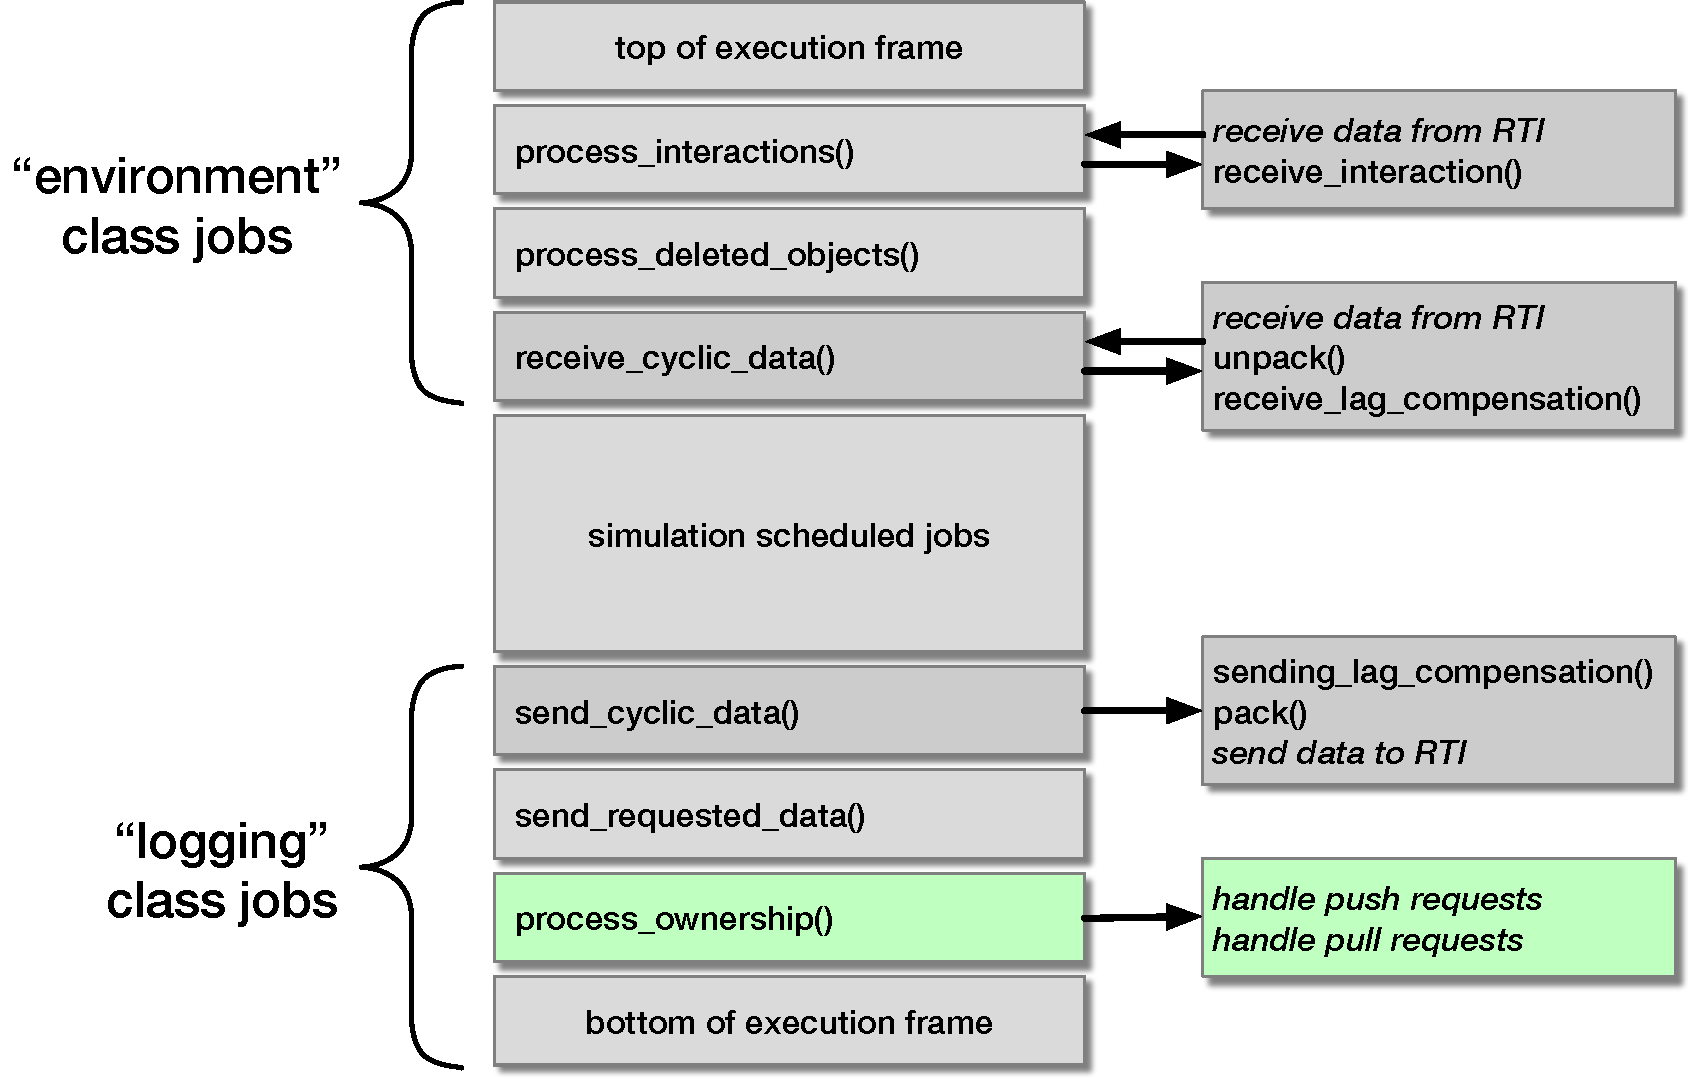
\includegraphics[scale=0.4]{TutorialTHLAOwnershipJobs.pdf}
      \end{figure}
   \end{frame}

   \begin{frame}
      \frametitle{Ownership Transfer}
      \framesubtitle{PITFALL - Handling Mixed Ownership}
      \begin{itemize}
         \item With ownership transfer, it is possible to have an object
         containing attributes you own and attributes you don’t own.
         \item TrickHLA knows to only send attributes you own, and only receive
         attributes you don’t own. However \ldots
         \item Your \texttt{unpack()} or \texttt{receive\_lag\_compensation()}
         functions run AFTER TrickHLA receives data, so they could accidently
         override your simulation state for attributes that you own and publish.
         This results in corrupted simulation data!
         \item To avoid overriding your simulation state, the solution is to
         determine if the attribute is owned by another federate in your
         \texttt{unpack()} and \texttt{receive\_lag\_compensation()} functions.
      \end{itemize}
      \begin{footnotesize}
      NOTE: the same scenario for your \texttt{pack()} or
      \texttt{send\_lag\_compensation()} functions is not a problem because
      they run BEFORE TrickHLA sends data, and because TrickHLA will not
      send data you don’t own, no harm done.
      \end{footnotesize}
         
   \end{frame}

   \begin{frame}[fragile]
      \frametitle{Ownership Transfer}
      \framesubtitle{PITFALL - Handling Mixed Ownership in Unpacking}
      \begin{itemize}
         \item Step 1: Add a \texttt{TrickHLA::Attribute} reference for each of
         your simulation state attributes. Example in \texttt{SinePacking.hh}:
      \end{itemize}
\begin{Verbatim}[frame=single, fontsize=\tiny]
   #include ”SineData.hh”
   #include "TrickHLA/include/TrickHLAAttribute.hh”
   #include "TrickHLA/include/TrickHLAPacking.hh”

   class SinePacking : public TrickHLAPacking
   {
     public:
      …
      // Initialize the packing object.
      void initialize( SineData * sim_data );
      // From the TrickHLAPacking class.
      virtual void initialize_callback( TrickHLAObject * obj );

      // From the TrickHLAPacking class.
      virtual void pack();
      // From the TrickHLAPacking class.
      virtual void unpack();

     private:
      SineData * sim_data; // -- Simulation data.
      double phase_deg;    // d  Phase offset in degrees.

      TrickHLAAttribute * phase_attr; // ** Reference to Phase TrickHLAAttribute.
   };
\end{Verbatim}
   \end{frame}

   \begin{frame}[fragile]
      \frametitle{Ownership Transfer}
      \framesubtitle{PITFALL - Handling Mixed Ownership in Unpacking (Continued)}
      \begin{itemize}
         \item Step 2: Override the \texttt{initialize\_callback()} function to
         set the attribute references.
         \item Example in \texttt{SinePacking.cpp}:
      \end{itemize}
\begin{Verbatim}[frame=single, fontsize=\scriptsize]
void SinePacking::initialize_callback( // RETURN: -- None.
   TrickHLAObject * obj ) // IN: -- Object associated with this packing class.
{
   // We must call the original function so that the callback is initialized.
   this->TrickHLAPacking::initialize_callback( obj );

   // Get a reference to the TrickHLAAttribute for the "Phase" FOM attribute.
   // We do this here so that we only do the attribute lookup once instead of
   // looking it up every time the unpack function is called.
   phase_attr = get_attribute_and_validate( "Phase" );
}
\end{Verbatim}
   \end{frame}

   \begin{frame}[fragile]
      \frametitle{Ownership Transfer}
      \framesubtitle{PITFALL - Handling Mixed Ownership in Unpacking (Continued)}
      \begin{itemize}
         \item Step 3: Check the attribute ownership in the unpack() function.
      \end{itemize}
\begin{Verbatim}[frame=single, fontsize=\scriptsize]
void SinePacking::unpack() // RETURN: -- None.
{
   // If the HLA phase attribute has changed and is remotely owned (i.e. is
   // coming from another federate) then override our simulation state with the
   // incoming value. If we locally own the "Phase" attribute then we do not
   // want to override it's value. If we did not do this check then we would be
   // overriding state of something we own and publish with whatever value
   // happen to be in the "phase_deg" local variable, which would cause data
   // corruption of the state. We always need to do this check because
   // ownership transfers could happen at any time or the data could be at a
   // different rate.
   if ( phase_attr->is_received() ) {
      // For this example to show how to use the Packing API's, we will
      // assume that the phase shared between federates is in degrees so
      // covert it back from degrees to radians.
      sim_data->set_phase( phase_deg * M_PI / 180.0 );
   }
}
\end{Verbatim}
   \end{frame}
   

   
   
   \section{Object Deletion}

   \begin{frame}
      \frametitle{Object Deletion}
      \begin{center}
      \Huge{Object Deletion}
      \end{center}
   \end{frame}
   
   \begin{frame}
      \frametitle{Object Deletion}
      \begin{itemize}
         \item TrickHLA supports notification of HLA object deletions.
         \item An HLA object can be deleted as a result of a federate resigning
         or by explicit deletion by the federate.
         \item Using TrickHLA object deletion consists of three steps:
         \begin{itemize}
            \item Step 1: Extend the \texttt{TrickHLA::ObjectDeleted} class
            and implement the \texttt{deleted()} virtual function.
            \item Step 2: In the \texttt{S\_define} file add an object-deleted
            object to each simulation object that needs to be notified of a
            deletion.
            \item Step 3: Configure object deleted in the \texttt{input.py} file.
         \end{itemize}
      \end{itemize}
   \end{frame}

   \begin{frame}[fragile]
      \frametitle{Ownership Transfer}
      \framesubtitle{Step 1: Extend the \texttt{TrickHLA::ObjectDeleted} Class}
      \begin{itemize}
         \item Step 1: Extend the \texttt{TrickHLA::ObjectDeleted} class and
         implement the \texttt{deleted()} virtual function.
         \item Example in \texttt{SineObjectDeleted.hh}:
      \end{itemize}
\begin{Verbatim}[frame=single, fontsize=\scriptsize]
#include "TrickHLA/include/TrickHLAObjectDeleted.hh”

class SineObjectDeleted : public TrickHLAObjectDeleted
{
...
  public:
...
   void deleted(                // RETURN: -- None.
        TrickHLAObject * obj ); // IN:     -- Deleted object.
};
\end{Verbatim}
   \end{frame}

   \begin{frame}[fragile]
      \frametitle{Ownership Transfer}
      \framesubtitle{Step 1: Extend the \texttt{TrickHLA::ObjectDeleted} Class (Continued)}
      \begin{itemize}
         \item Step 1 continued: Example in \texttt{SineObjectDeleted.cpp}:
      \end{itemize}
\begin{Verbatim}[frame=single, fontsize=\scriptsize]
void SineObjectDeleted::deleted( // RETURN: -- None.
   TrickHLAObject * obj)         // IN: -- Object which was deleted.
{
   std::ostringstream msg;
   msg << "SineObjectDeleted::deleted() Object '" << obj->get_name()
       << "' deleted from the federation.";
   send_hs( stdout, (char *) msg.str().c_str() );
}
\end{Verbatim}
   \end{frame}

   \begin{frame}[fragile]
      \frametitle{Ownership Transfer}
      \framesubtitle{Step 2: Add Object-deleted Object to \texttt{S\_define}}
      \begin{itemize}
         \item Step 2: In the \texttt{S\_define} file add an object-deleted
         object to each simulation object that needs to be notified of a deletion.
      \end{itemize}
\begin{Verbatim}[frame=single, fontsize=\scriptsize]
   class ASimObject : public Trick::SimObject {
      ...
      SineData     sim_data;
      SineData     lag_comp_data;
      SineOwnershipHandler   ownership_handler;
      SinePacking            packing;
      SineLagCompensation    lag_compensation;
      SineInteractionHandler interaction_handler;
      SineObjectDeleted      obj_deleted_callback;

      ASimObject() {
        P50 ("initialization") packing.initialize( &sim_data );
        P50 ("initialization") lag_compensation.initialize( &sim_data, 
                                                            &lag_comp_data );
        ...
      }
   };
\end{Verbatim}
   \end{frame}

   \begin{frame}[fragile]
      \frametitle{Ownership Transfer}
      \framesubtitle{Step 3: Configuration}
      \begin{itemize}
         \item Step 3: Configure object deleted in the \texttt{input} file.
         \item In the \texttt{RUN\_a\_side/input.py} file:
\begin{Verbatim}[frame=single, fontsize=\scriptsize]
THLA.manager.objects[0].deleted = A.obj_deleted_callback
THLA.manager.objects[1].deleted = P.obj_deleted_callback
\end{Verbatim}
         \item In the \texttt{RUN\_p\_side/input.py} file:
\begin{Verbatim}[frame=single, fontsize=\scriptsize]
THLA.manager.objects[0].deleted = A.obj_deleted_callback
THLA.manager.objects[1].deleted = P.obj_deleted_callback
\end{Verbatim}
      \end{itemize}
   \end{frame}
   
   \begin{frame}
      \frametitle{Object Deletion}
      \framesubtitle{TrickHLA jobs in THLA.sm}
      \begin{figure}
      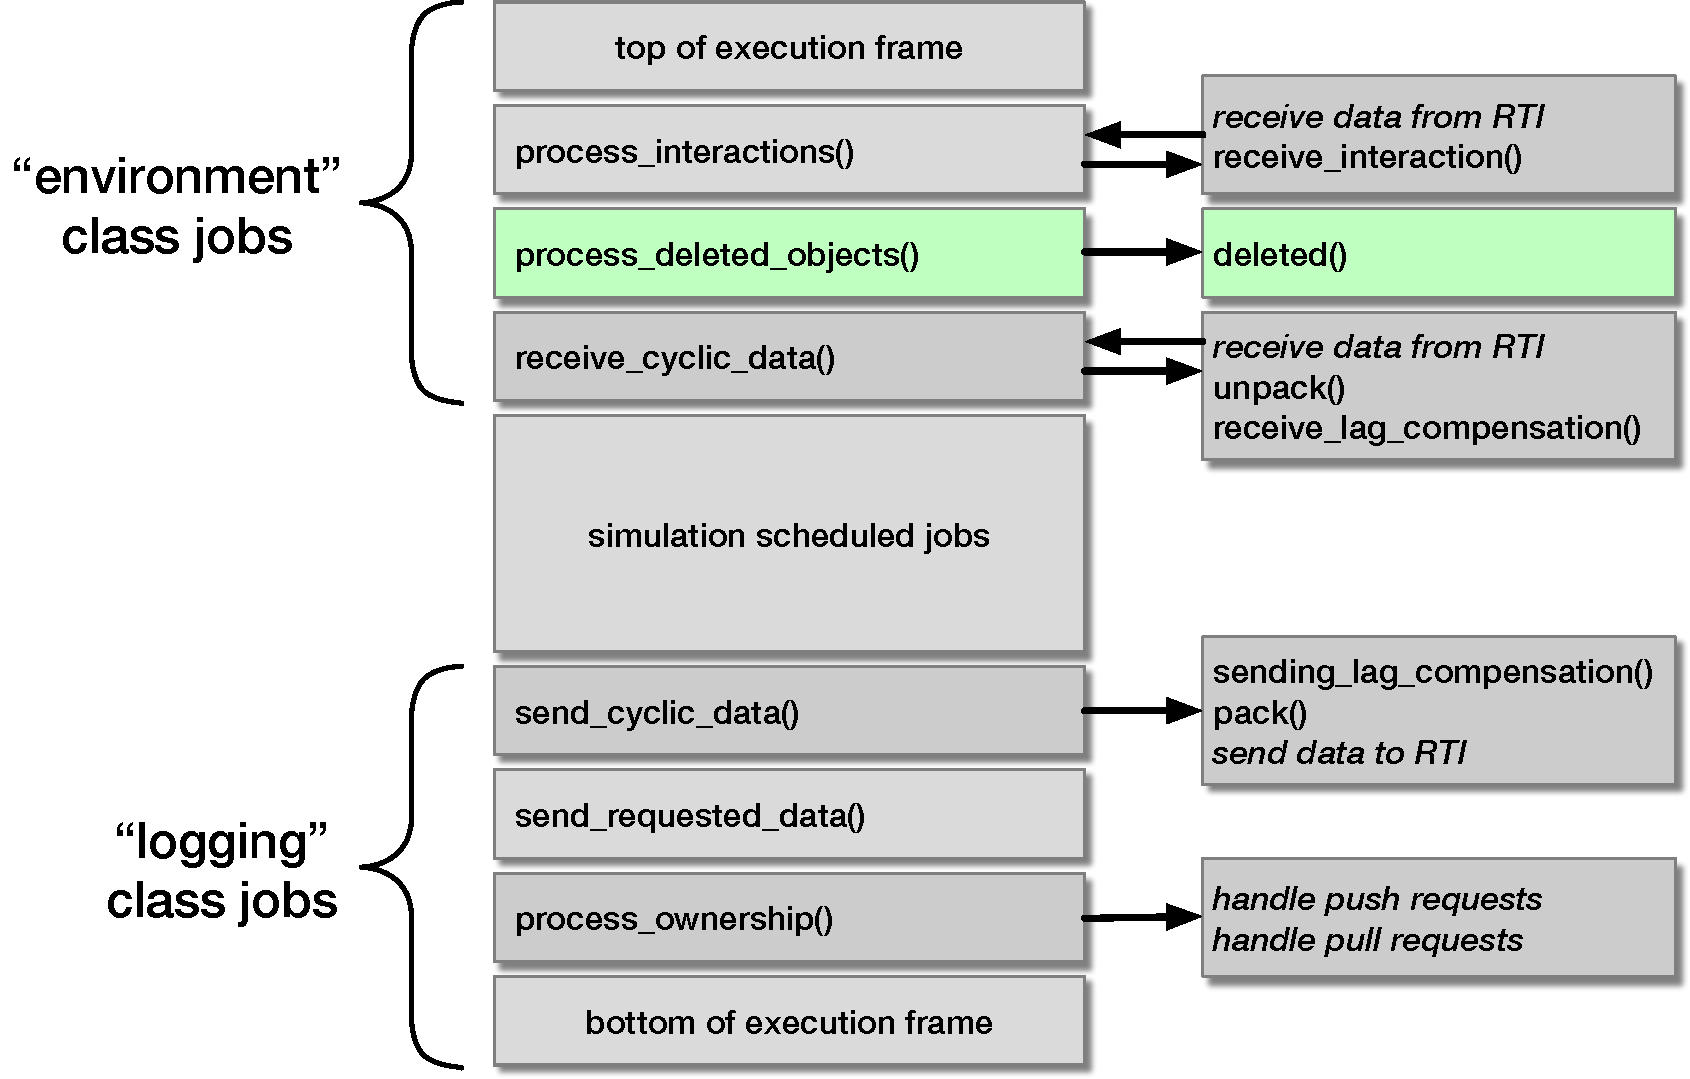
\includegraphics[scale=0.4]{TutorialTHLADeletedJobs.pdf}
      \end{figure}
   \end{frame}


   \begin{frame}
      \titlepage
   \end{frame}
   
\end{document}
